\chapter{Diskretizace tunelu}

Tunel $ \Tau $ v molekule je v našem případě modelován posloupností koulí o různých
poloměrech umístěných v prostoru. Pro posloupnost koulí $ \Tau = \{S_i\}_{i=0}^{n} $
musí platit

    \begin{enumerate}[label={(\arabic*)}]
        \item $ S_i \bigcap S_{i+1} \neq \emptyset $ pro všechna $ 0 \leq i < n$,
        \item $ S_i \nsubseteq S_j$  pro $ i \neq j $.
    \end{enumerate}

K tomu ještě budeme požadovat, aby tunel sám sebe nikdy neprotínal. Exaktněji řečeno
chceme, aby byl objem tunelu $ \Tau $ homeomorfní s objemem válce v topologickém smyslu.
Pro představu, jak takový tunel může vypadat, uvádíme obrázek \ref{fig:basic_tunnel}.
\begin{figure}[ht]
    \centering
    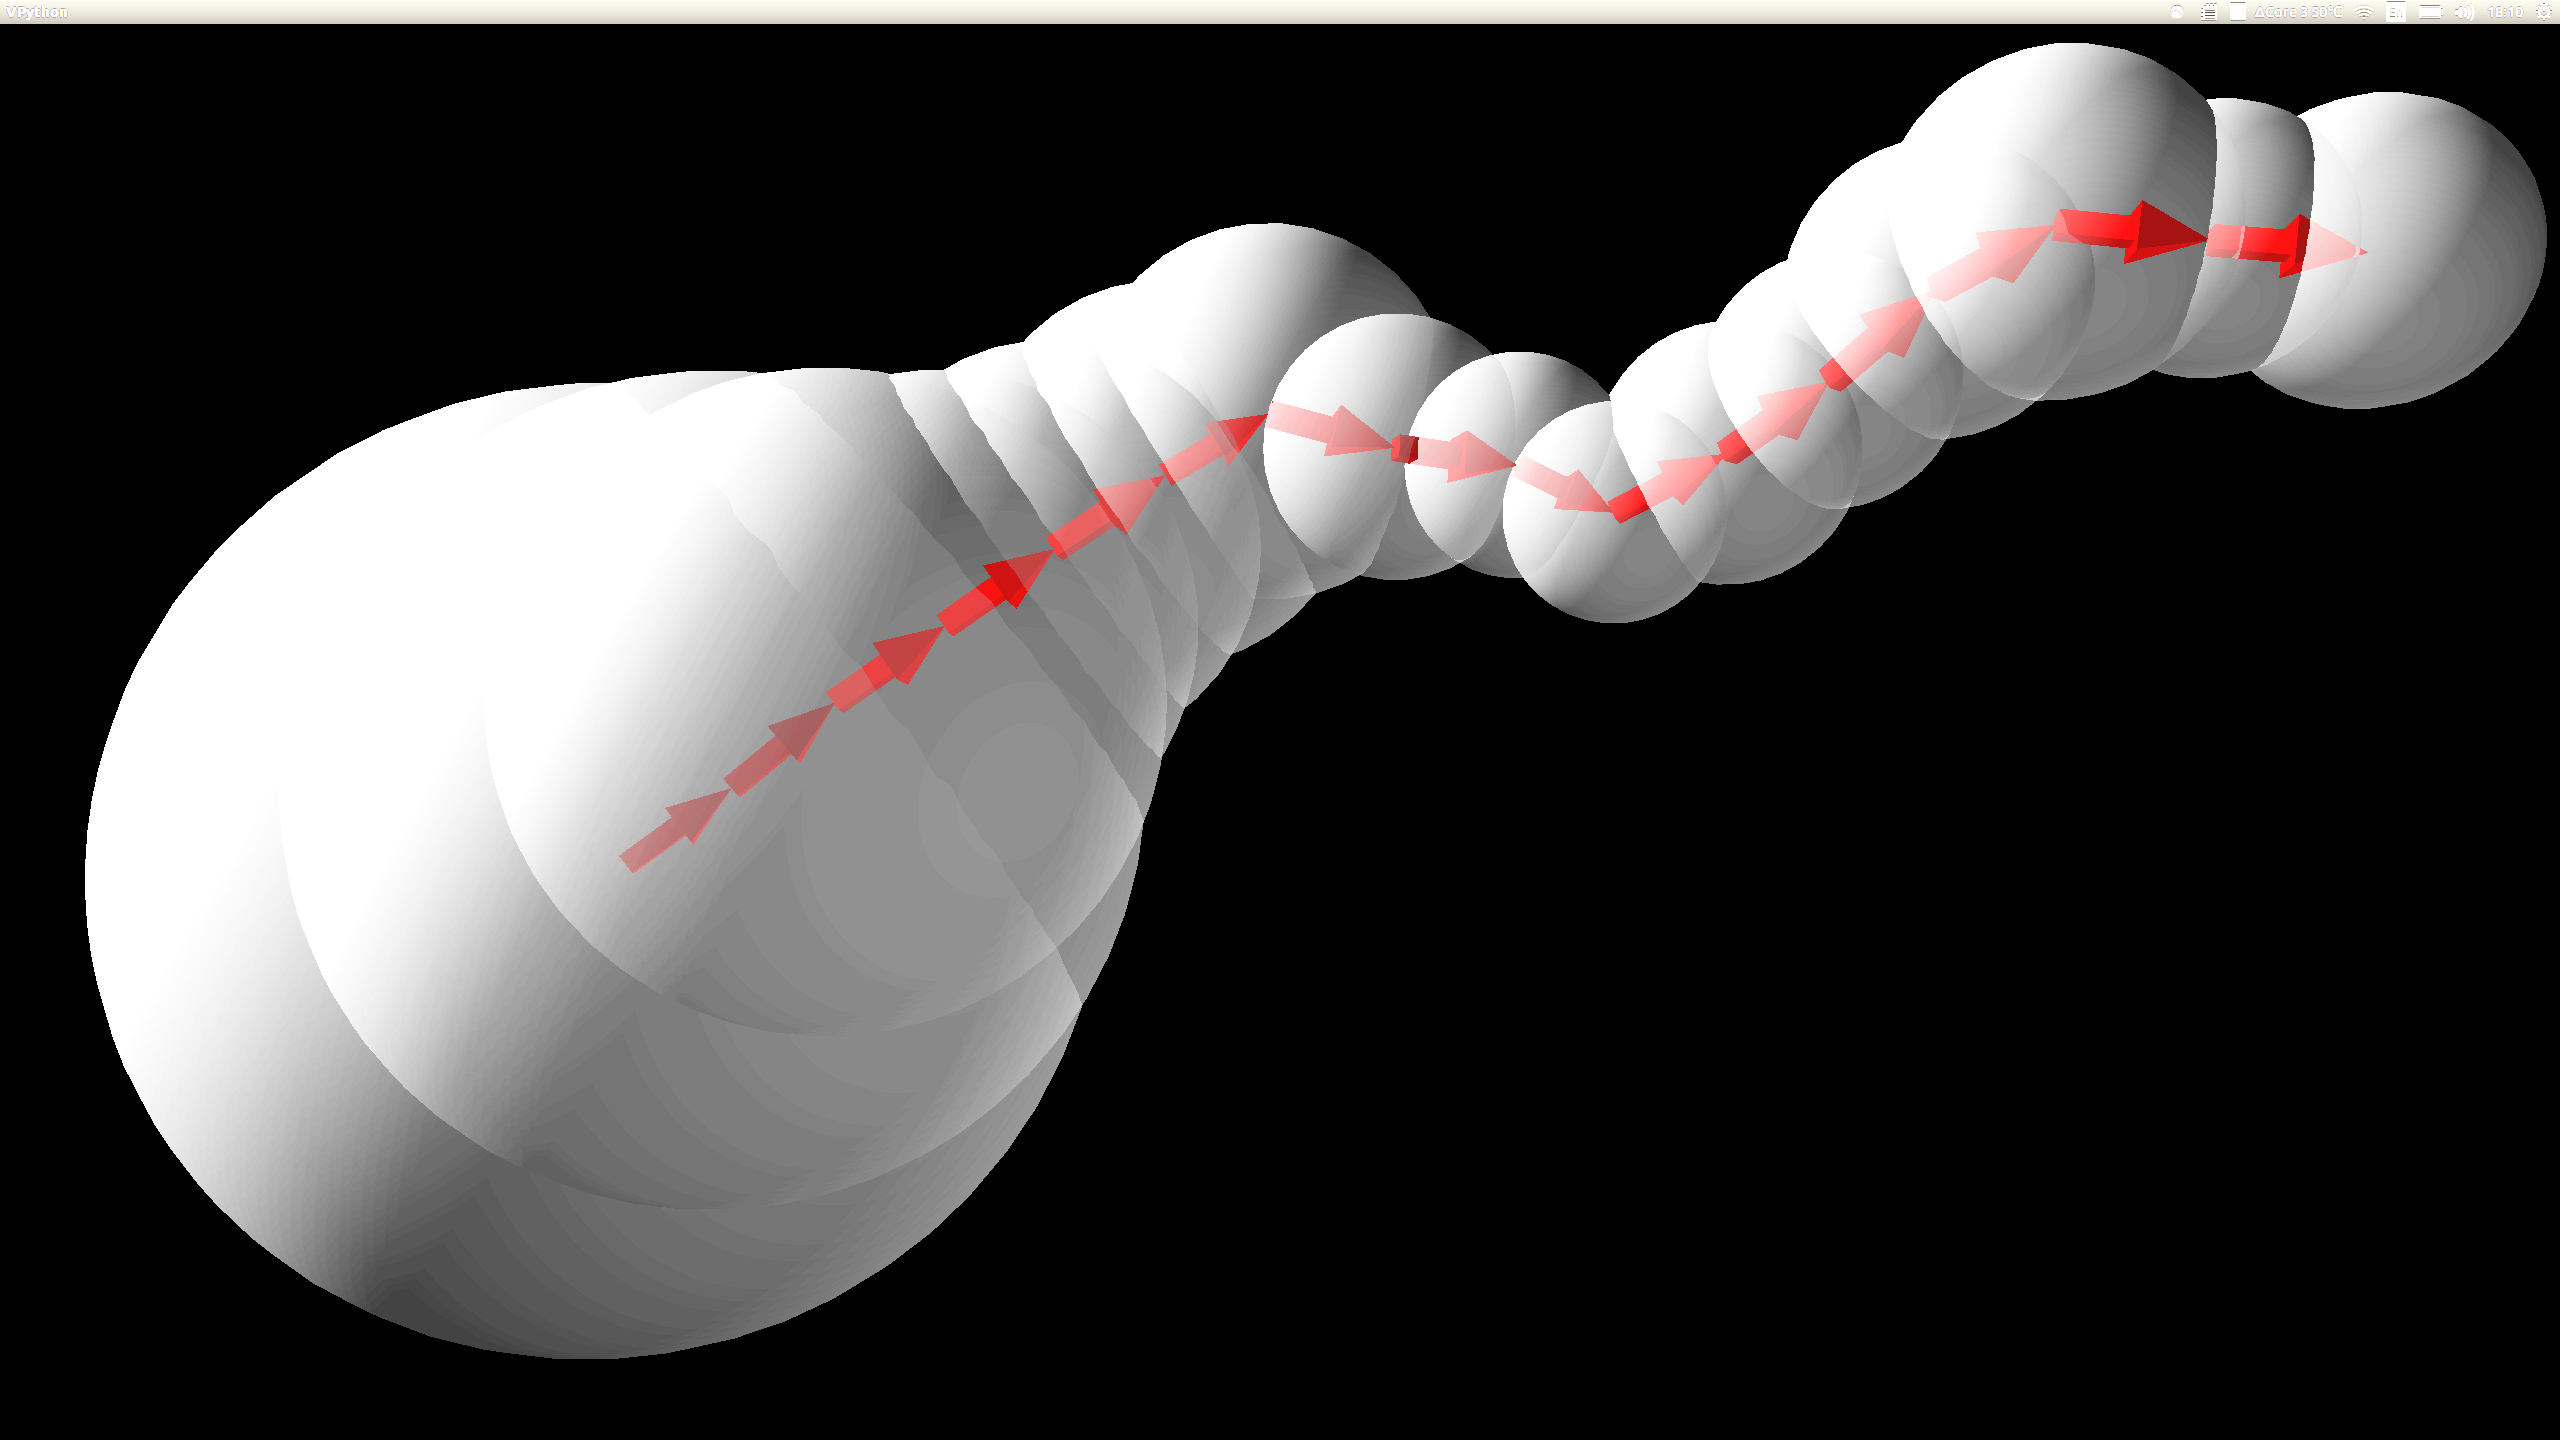
\includegraphics[width=100mm]{img/basic_tunnel.jpg}
    \caption{Tunel v molekule}
  \centering
  \label{fig:basic_tunnel}
\end{figure}

Na mnohých místech budeme potřebovat mluvit o takzvané trajektorii tunelu. Tu popisuje
následující definice.

\begin{defi}
Mějme tunel $ \Tau $. Trajektorií tunelu $ \Tau $ budeme rozumět křivku tvořenou
úsečkami danými dvojicemi středů po sobě jdoucích koulí $ S_i^{center} $,
$ S_{i+1}^{center} $ pro $ 0 \leq i < n$.
\end{defi}

Abychom mohli provádět doking ligandu, musíme nejprve takto definovaný tunel nařezat na
jemné plátky – kruhy, na které pak budeme v průběhu výpočtu dokovat průběžné konformace ligandu.
Popišme si nyní, jak by takové řezy měly vypadat.

\begin{defi}
Řezem tunelu $ \Tau $ rozumíme kruh v prostoru, který je určen uspořádanou trojicí
$\theta = (A, u, r)$, kde $ A $ je střed, $ u \in \Rbb^3 $ je normálový vektor a $ r > 0 $ je poloměr.
Pro tento kruh $ \theta $ musí platit, že $ \Tau \cap \theta $ je souvislá množina a navíc
$ \exists \delta > 0 $ tak, že $ \forall \varepsilon > 0,  \varepsilon < \delta $ je
$ (A, u, r + \varepsilon) \cap \Tau = \theta \cap \Tau $.
(Alternativně řečeno $\Tau \setminus \theta $ má dvě komponenty souvislosti.)
\end{defi}

Uvedená definice prakticky říká, že řez tunel řeže jen na jednom místě (podmínka souvislosti).
Druhá podmínka znamená, že řez je úplný, tedy že řezem skutečně rozdělíme tunel na dvě části.
Pro ilustraci, jak takové řezy mohou vypadat, přikládáme obrázek č. \ref{fig:tunnel_cuts}.
\begin{figure}[ht]
    \centering
    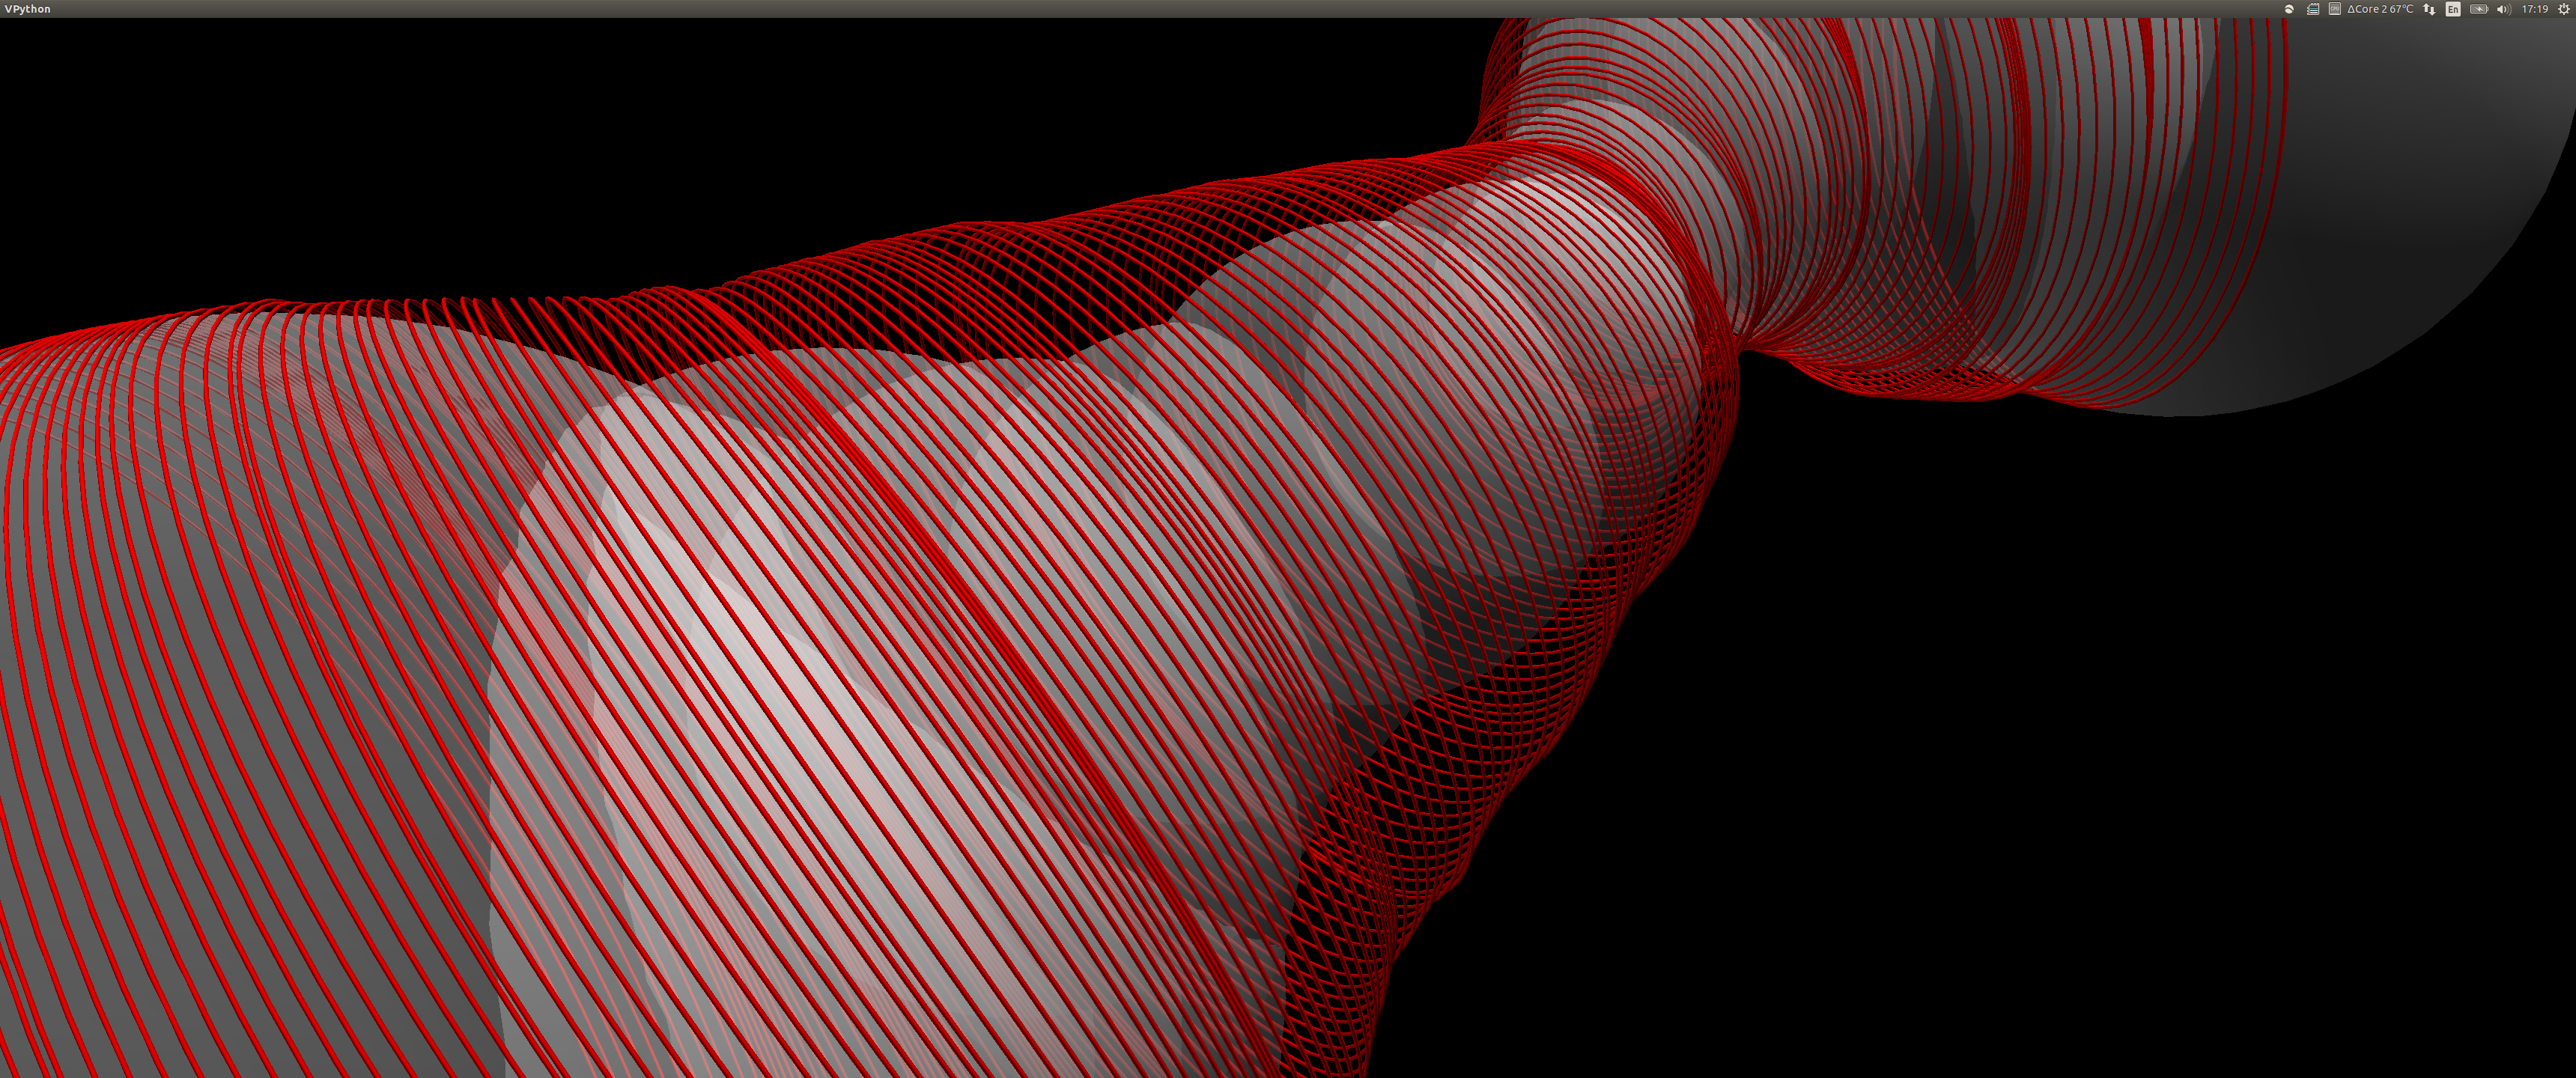
\includegraphics[width=\textwidth]{img/simple_cuts.png}
    \caption{Řezy}
  \centering
  \label{fig:tunnel_cuts}
\end{figure}

S takto definovanými řezy můžeme začít uvažovat o tom, jak tunel nařezat jako celek.
Mějme $ \Theta = \{\theta_i\}_{i=0}^{k}$ posloupnost řezů tunelu $ \Tau $. Pro potřeby správného
dokingu bude nezbytné, aby platilo

\begin{align}
x, y \in \Theta \Rightarrow |x \cap y| \leq 1, \label{cond:not_intersecting}
\end{align}

tedy každé dva řezy se dotýkají nejvýše v jednom bodě. Dále budeme chtít, aby vzdálenost
po sobě jdoucích řezů byla shora omezená. Vzdálenost budeme měřit pomocí funkce
$ \dst(x, y) $, kterou popisuje následující definice.

\begin{defi}
Mějme řezy $ x = (A, u, r_1), y = (B, v, r_2) \in \Theta $. Vzdálenost řezů budeme
měřit v jejich projekci do roviny $ \rho = (A, u, w) $, určenou středem $ A $,
vektorem $ u $ a druhým vektorem $ w $, který definujeme následovně:
    \begin{enumerate}[label={(\arabic*)}]
        \item Pokud jsou vektory $ u $, $ v $ a $ A - B $ po dvou lineárně závislé (LZ), vezmeme
            za $ w $ libovolný nenulový vektor lineárně nezávislý (LN) na $ u $.
        \item V případě, že $ u $, $ v $ jsou LZ ale $ u $ a $ A - B $ jsou LN,
            definujeme $ w = A - B $.
        \item Jinak položíme $ w = v $.
    \end{enumerate}
Kolmým promítáním řezů $ x $, resp. $ y $ do roviny  $ \rho $ získáme dvě úsečky
určené vrcholy $X_1, X_2 $, resp. $Y_1, Y_2 $. Vzdálenost pak definujeme jako
\begin{center}
    $ \dst(x, y) = \min\{ \max\{|X_1 - Y_1|, |X_2 - Y_2|\}, \max\{|X_1 - Y_2|, |X_2 - Y_1|\}\}$.
\end{center}
\end{defi}

Uvedená definice je nezávislá na volbě vektoru $ w $ v podmínce (1), neboť
v této situaci jsou řezy zarovnány přesně za sebou a pro libovolnou rovinu
kolmou na oba řezy dostaneme stejné projekční úsečky.

Vzdálenost $ \dst $ použijeme k formulaci následující podmínky:
\begin{align}
    \theta_i, \theta_{i+1} \in \Theta \Rightarrow \dst(\theta_i, \theta_{i+1}) < \delta.
    \label{cond:distance}
\end{align}


Přirozeným požadavkem je, abychom se tunelem pohybovali stále vpřed.
Vzhledem k tomu, že řez $ \theta_i \in \Theta $ musí dělit tunel vždy na dvě části, stačí
požadovat, aby střed následujícího řezu $ \theta_{i + 1} \in \Theta $ ležel před
$ \theta_i $. To zajistíme podmínkou \ref{cond:going_forward}.

\begin{align}
    \theta_i, \theta_{i+1} \in \Theta
        \Rightarrow \langle \theta_i^{normal}, \theta_{i+1}^{center} - \theta_i^{center} \rangle > 0
        \label{cond:going_forward}
\end{align}
Poznamenejme, že $ \langle \cdot, \cdot \rangle$ značí skalární součin.
Nakonec přidáním podmínky \ref{cond:good_start} na první a poslední řez zajistíme,
že řezy pokryjí tunel v celé jeho délce. Pro potřeby této podmínky označme
$ w = S_2^{center} - S_1^{center} $.

\begin{align}
    \theta_1^{normal} = \frac{w}{\norm{w}}
    \qquad  \qquad S_1^{center} \in \theta_1
    \qquad  \qquad S_n^{center} \in \theta_k
    \label{cond:good_start}
\end{align}

Nyní můžeme přistoupit k popisu samotného algoritmu, který má na vstupu tunel $ \Tau $
a nějaké pevně zadané $ \delta > 0$, které určuje maximální vzdálenost, kterou
od sebe dva po sobě jdoucí řezy mohou mít. Na výstupu pak budeme očekávat řezy pokrývající
celý tunel a budou splňovat uvedené omezení na vzdálenost. Vzhledem k tomu, že výsledná
složitost následného dokingu je přímo úměrná počtu řezů, budeme od algoritmu chtít,
aby počet řezů byl při splnění uvedených kritérií pokud možno co nejmenší.


\section{Algoritmus}

Celý algoritmus se sestává z celé řady funkcí řešících více či méně důležité podproblémy.
Domníváme se, že vyčerpávající popis všech komponent by byl zbytečně technický,
proto se zde zaměříme zejména na popis těch opravdu klíčových
a tam, kde implementace nějakého výpočtu nebude důležitá pro pochopení fungování
algoritmu jako celku, se omezíme pouze na symbolický zápis, případně stručný slovní
popis.

Pro začátek si řekněme něco o základní kostře algoritmu. Přirozeným naivním přístupem
k řešení našeho problému, by bylo vzít trajektorii tunelu tvořenou středy koulí
jím definované, po této trajektorii se s krokem $ \delta $ posouvat a generovat
řezy se středem na trajektorii a normálou určenou směrem pohybu na trajektorii.
Takovýto přístup by fungoval vcelku dobře pro tunely, které by byly relativně
přímé bez zatáček, avšak pro \say{klikaté} tunely by generoval řezy zcela nepoužitelné.
Pro ilustraci uvádíme obrázek \ref{fig:naive_cuts}.

\begin{figure}
    \centering
    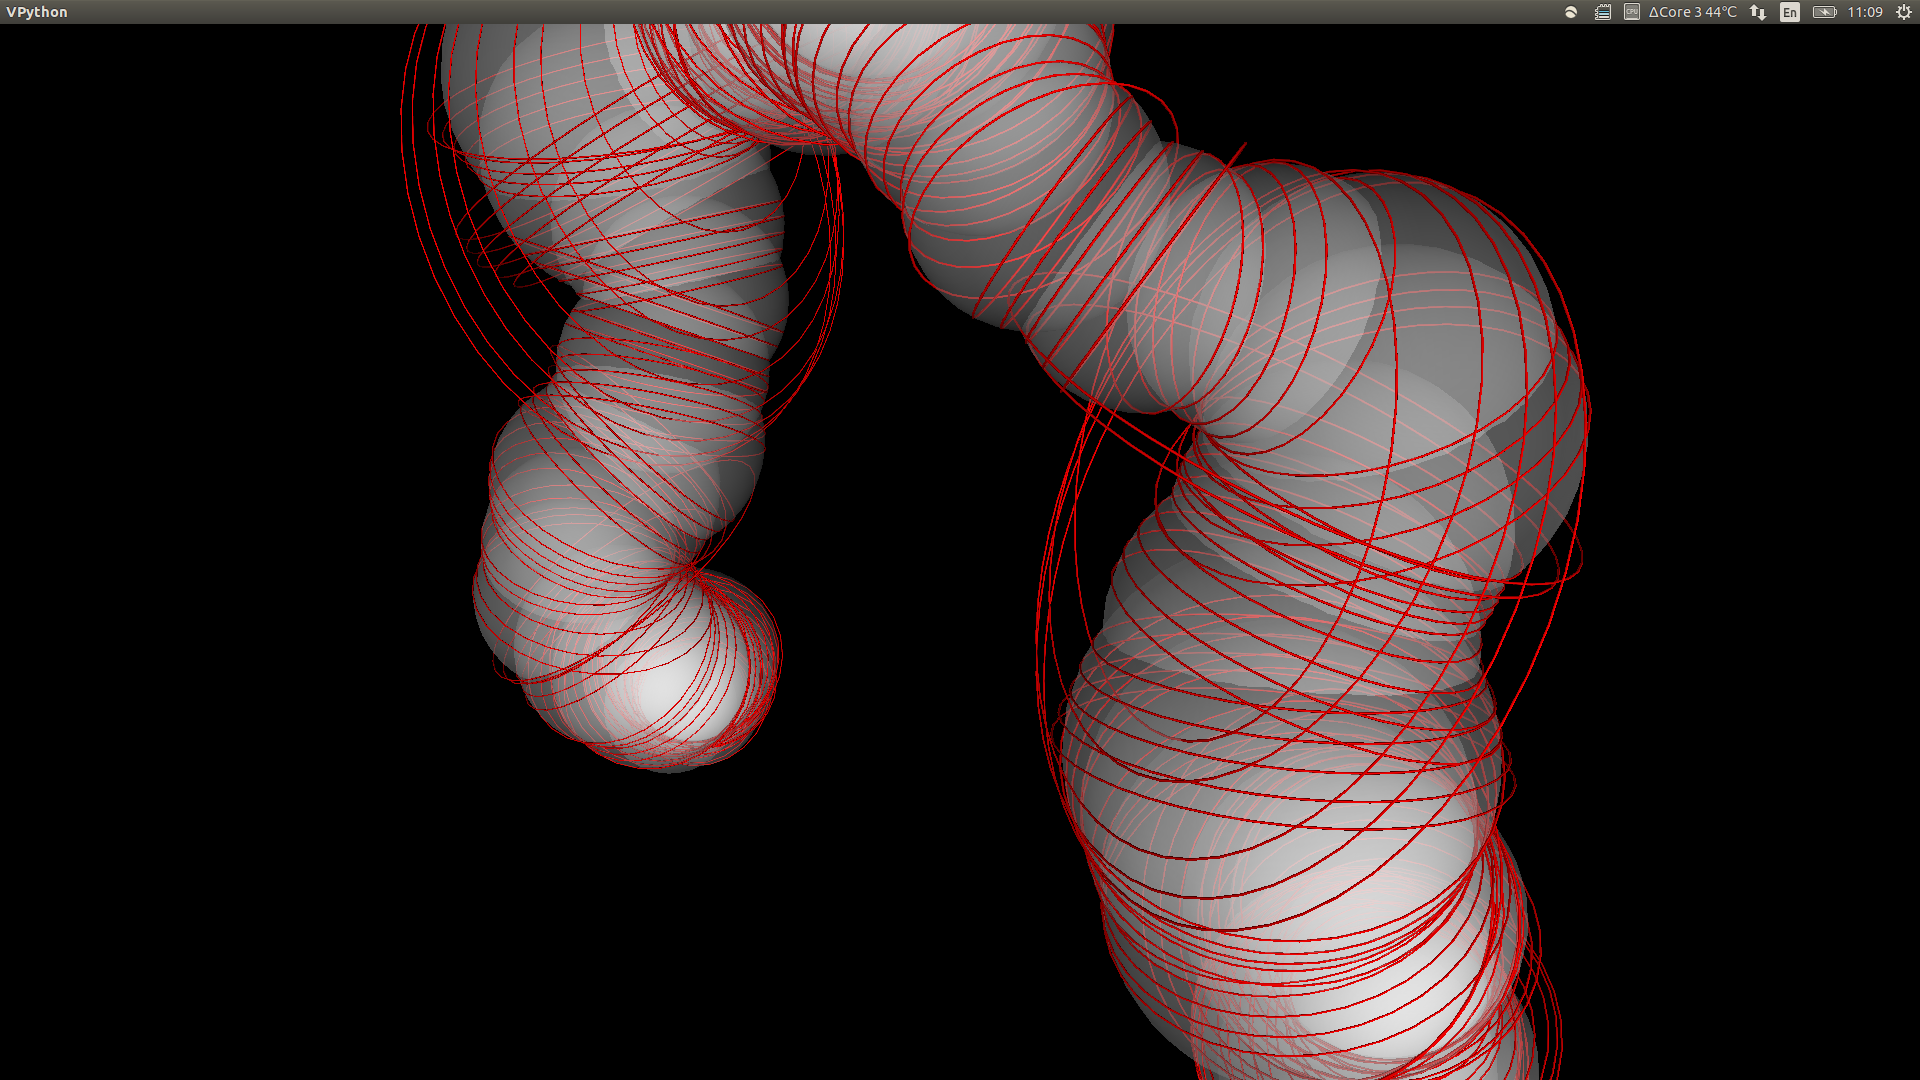
\includegraphics[width=\textwidth]{img/naive_cuts.png}
    \caption{Naivní řezy}
  \centering
  \label{fig:naive_cuts}
\end{figure}

K problémům dochází proto, že takto bereme v potaz pouze velmi lokální informace o vlastnostech
tunelu a zřejmě zcela ignorujeme dříve uvedené požadavky na řezy. Tento postup ale
můžeme zdokonalit. Prvním problémem je, že když takto postupně generujeme nové řezy,
může se stát, že od sebe budou příliš daleko nebo se budou protínat. Potřebujeme proto
funkci $ shiftDisk $, která přesně toto znemožní. Tuto funkci do detailu rozvedeme v
podkapitole \ref{subsec:disk_shift}. Ve stručnosti pouze poznamenejme, že tato funkce
vstupní řez upraví tak, aby neprotínal předchozí řez a byl od něj vzdálen nejvýše
o $ \delta $. Jak ale můžeme vidět na obrázku \ref{fig:shift_cuts}, toto způsobí,
že se v případě nevhodné orientace normálových vektorů sice zachovají naše
požadavky na řezy, avšak dostaneme jich zbytečně mnoho.

\begin{figure}
    \centering
    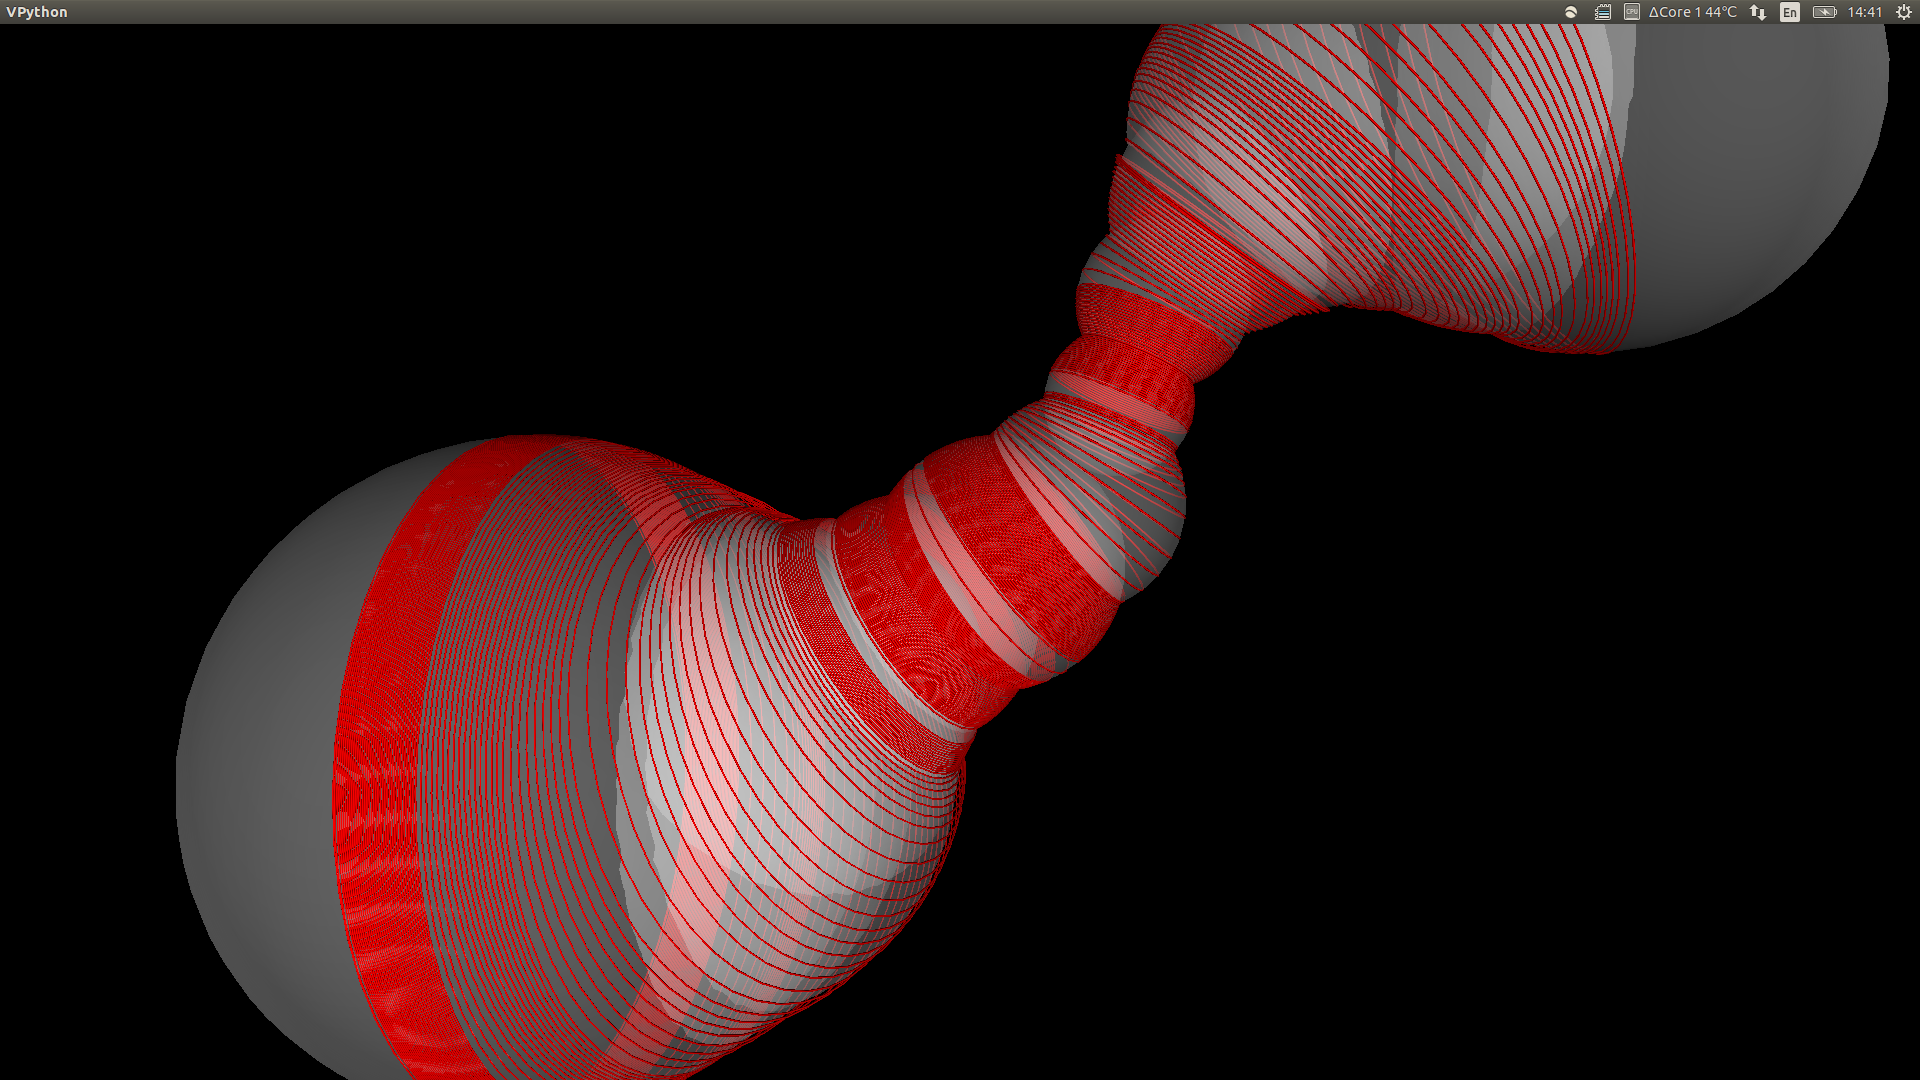
\includegraphics[width=\textwidth]{img/shift_cuts.png}
    \caption{Posun řezů}
  \centering
  \label{fig:shift_cuts}
\end{figure}

Z toho důvodu je ještě vhodné po každém posunu zkontrolovat, zda nemůžeme předchozí
řez vynechat. To jest pro $ \theta_{i - 2} \in \Theta $ zkontrolovat zda
náhodou neplatí $ \dst(\theta_{i - 2}, \theta) < \delta $. Jak můžeme vidět na
obrázku \ref{fig:cuts_with_replace}, výsledek již vypadá o mnoho lépe.

\begin{figure}
    \centering
    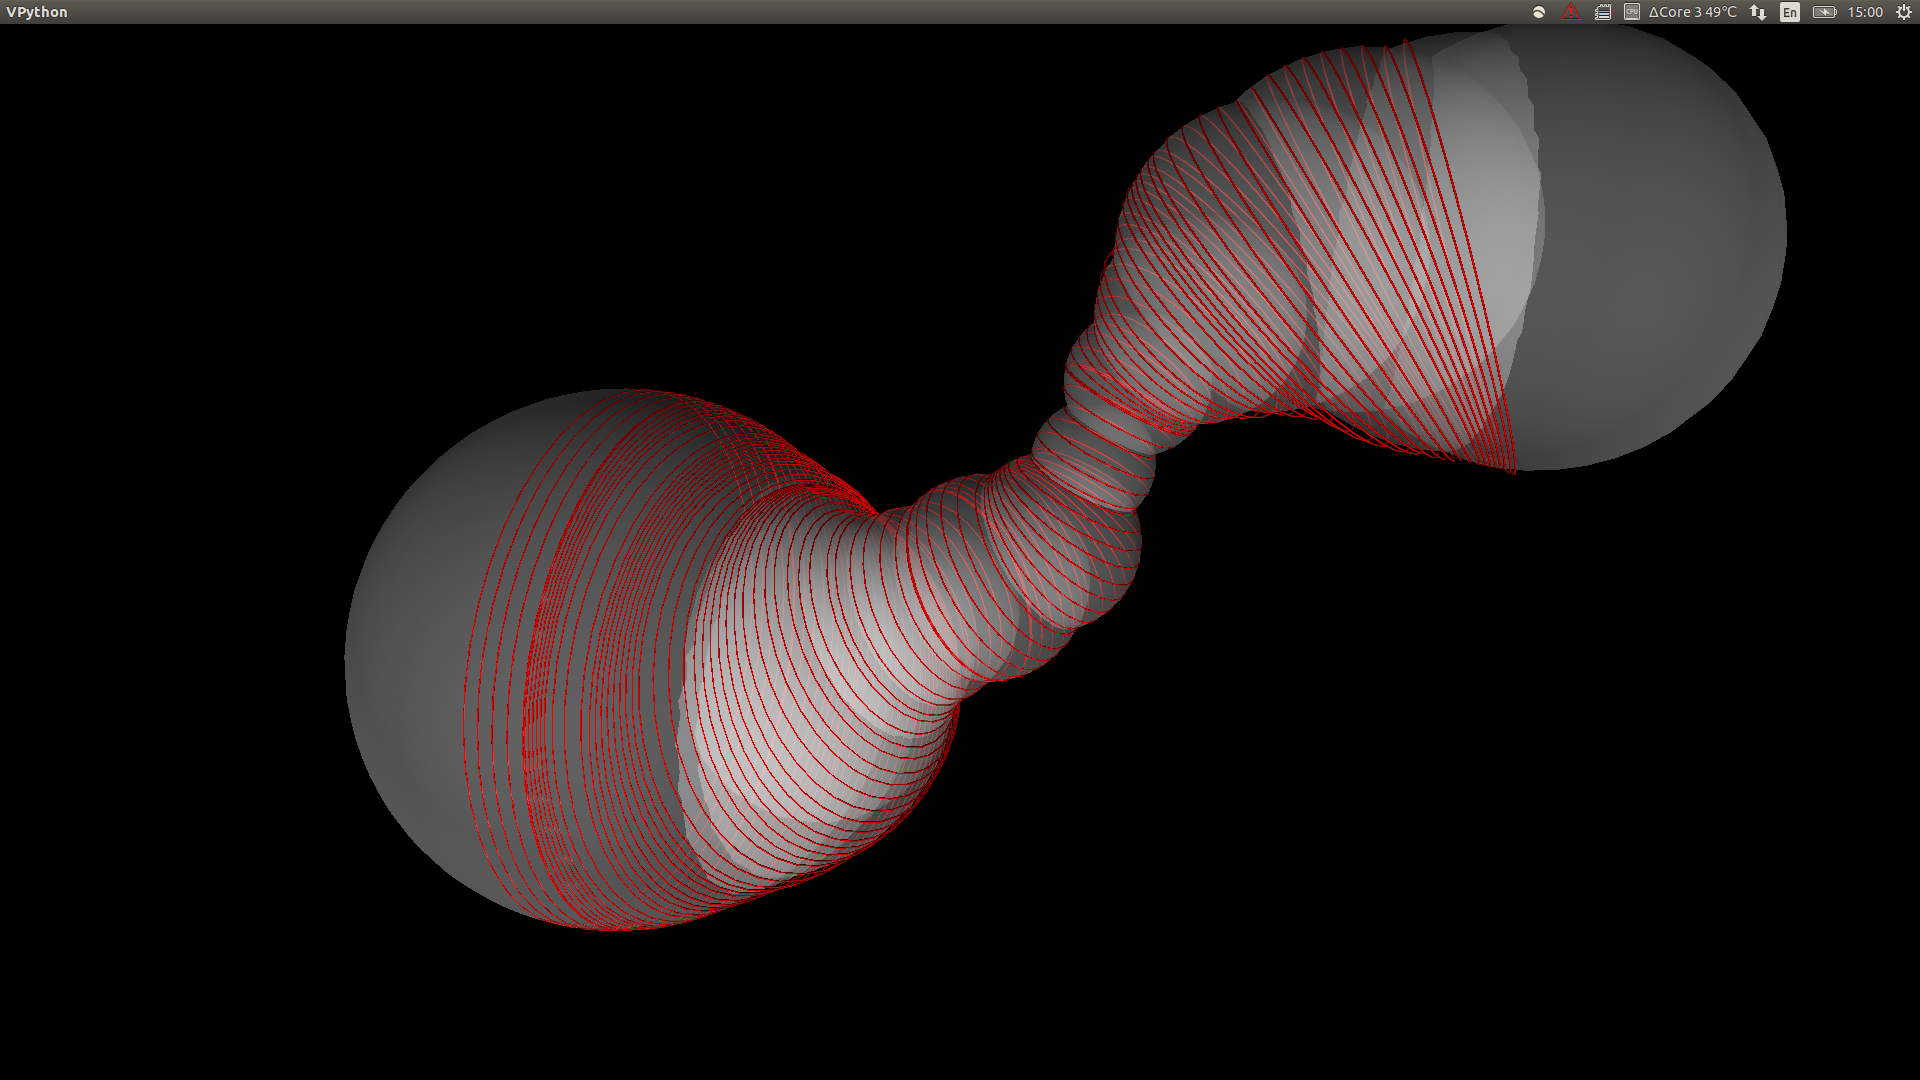
\includegraphics[width=\textwidth]{img/cuts_with_replace.png}
    \caption{Vynechání přebytečných řezů}
  \centering
  \label{fig:cuts_with_replace}
\end{figure}

Jak si ale pozorný čtenář může povšimnout, na pravém konci tunelu uvedeného na
posledním obrázku můžeme vidět, že řezy nezatáčí tak, jak by mohly, a nekopírují tak
profil tunelu příliš věrně. Po krátkém zamyšlení se dá nahlédnout, že tomu tak
je pravděpodobně kvůli tomu, jaké volíme výchozí normálové vektory pro jednotlivé
řezy. Pokud řezy orientujeme výhradně podle lokálních vlastností trajektorie,
tak se nám může stát, že právě například nezačneme zatáčet dostatečně brzy apod.
Z tohoto důvodu budeme pro výpočet normály nového řezu používat třídu
$ TunnelCurve $ a její metodu $ getWeightedDir $, která pro daný bod $ P $ na křivce
– trajektorii tunelu vrátí co nejlepší aproximaci směru tunelu na okolí bodu $ P $.
Exaktněji tento výpočet a případná zlepšení rozvedeme v podkapitole \ref{subsec:tunnel_dir}.
Pro ilustraci se ještě podívejme na obrázek \ref{fig:weighted_dir}. Je vidět, že
řezy nyní kopírují zakřivení tunelu mnohem ochotněji (neformálně řečeno jsou řezy
víc kolmé ke směru tunelu).

\begin{figure}[ht]
    \centering
    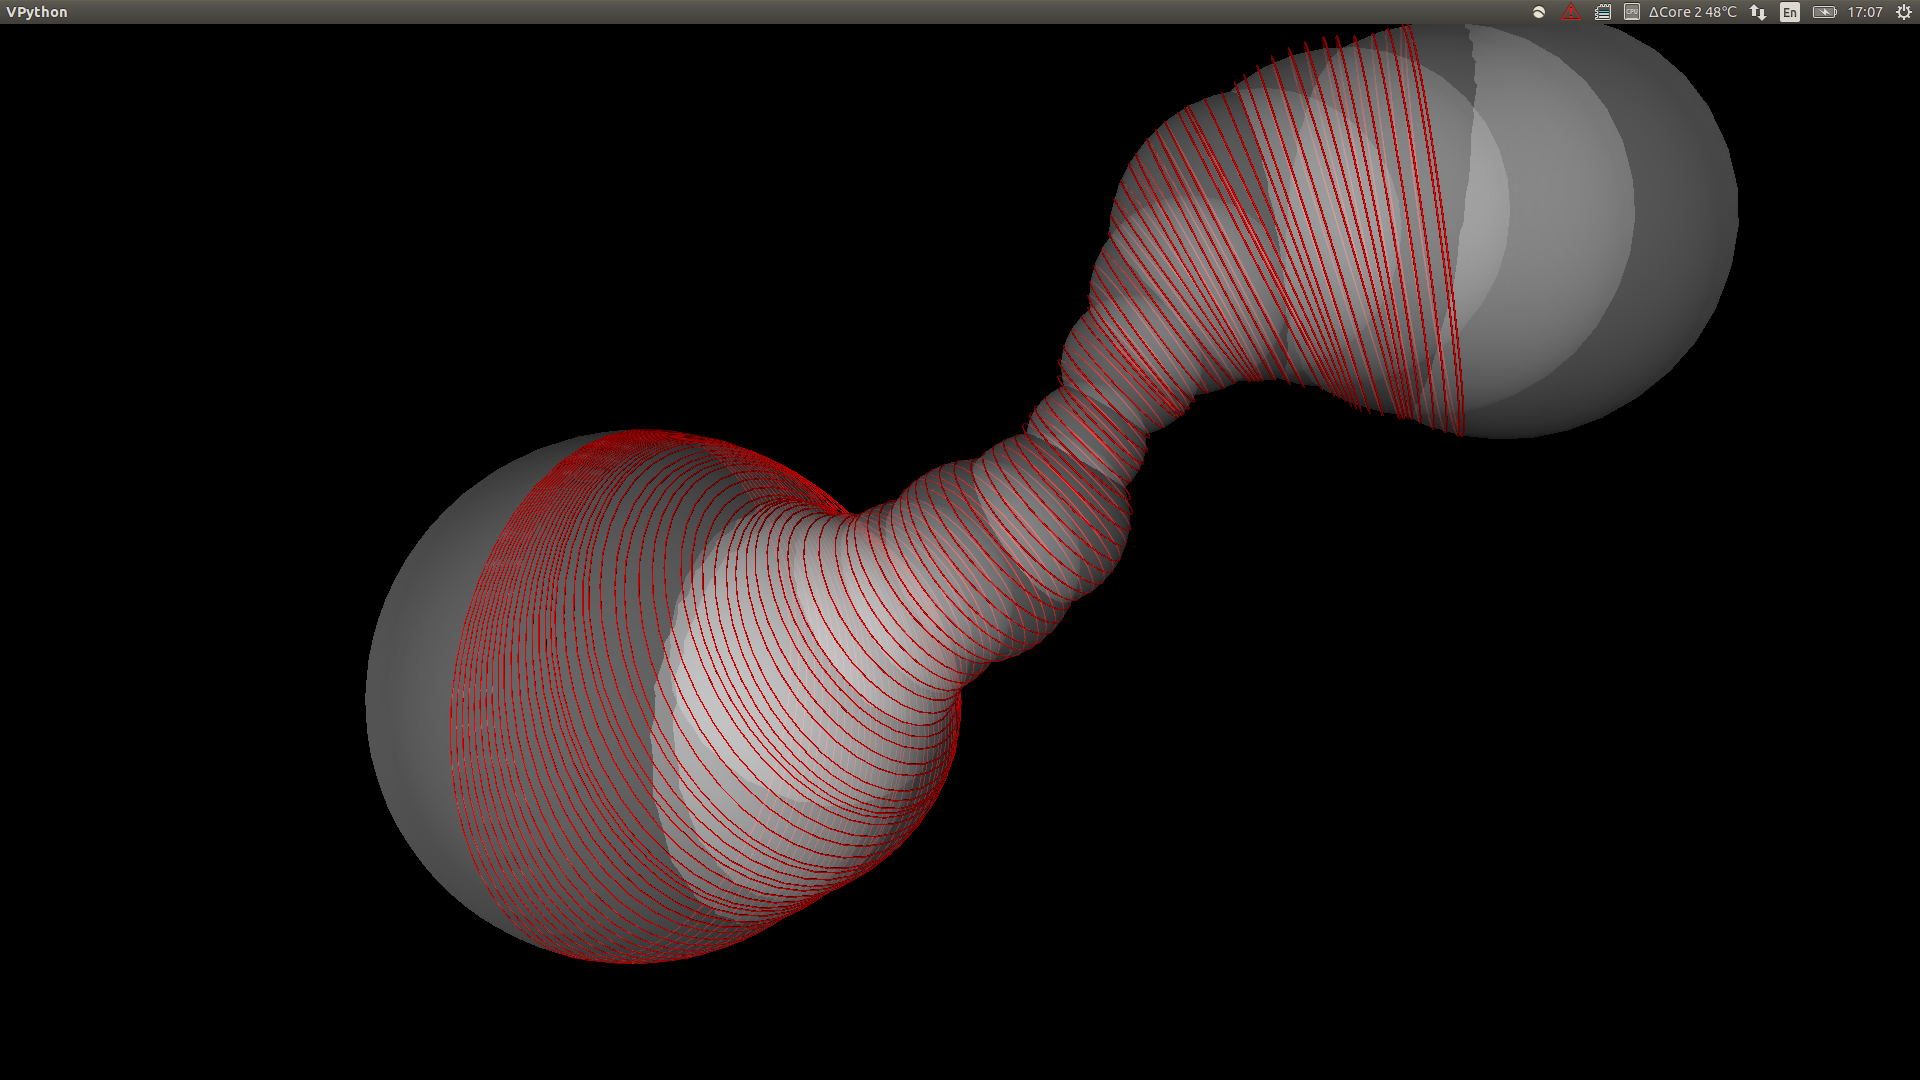
\includegraphics[width=\textwidth]{img/weighted_dir.png}
    \caption{Řezy s váženým průměrem směru}
  \centering
  \label{fig:weighted_dir}
\end{figure}

Takto formulovaný algoritmus fungoval obecně poměrně dobře, ale v případě tunelů,
které měly příliš prudké zatáčky nebo prudké změny v poloměru průřezu, často
selhával. Z tohoto důvodu jsme byli nuceni přidat ještě speciální proceduru
$ \operatorname{shiftToBend} $, která se aktivuje právě v těchto extrémních
případech. Podrobně se jí budeme věnovat v podkapitole \ref{subsec:shift_sharp_turn}.

Kostru naznačeného algoritmu zachycuje pseudokód č. \ref{alg:digTunnel}.
Poznamenejme, že budeme značit $ \operatorname{norm}(v) = \frac{v}{\norm{v}}$ a
výrazy \textit{pop}, resp. \textit{append} budeme používat pro odstranění posledního prvku z listu, resp.
přidání prvku na konec listu.

\begin{algorithm}
\caption{Algoritmus pro výpočet diskretizace tunelu}
\label{alg:digTunnel}
\begin{algorithmic}[1]

\Function{digTunnel}{$\Tau, \delta$}
    \State $ centers \gets [ S^{center} \mid S \in \Tau ] $ \label{digTunnel:first_init}
    \
    \State $ disks \gets   [ \operatorname{fitDiskTunnel}(\operatorname{norm}(S_{1}^{center} - S_{0}^{center}), S_0^{center})] $
    \State $ curve \gets \operatorname{TunnelCurve}(centers) $ \label{digTunnel:last_init}
    \Statex

    \For{$ S_i \gets S_0, \dots, S_{|T| - 2} $}
        \State $ dir \gets S_{i + 1}^{center} - S_{i}^{center} $
        \State $ line \gets \{ S_{i}^{center} + t\cdot dir \mid t \in \Rbb \} $

        \State $ d \gets 0 $
        \While {True}
            \State $ prev\_disk \gets disks[|disks|-1] $
            \State $ plane \gets \operatorname{getPlane}(prev\_disk) $ \Comment{Konstrukce roviny, ve které řez leží}
            \State $ d \gets \dis(plane \cap line, S_{i}^{center}) + \epsilon  $
            \If {$ d > \norm{dir} $} \label{digTunnel:while_condition}
                \Break
            \EndIf
            \Statex

            \If{$\operatorname{makesSharpTurn}(prev\_disk, curve)$}
                \State $ disk\_center
                    \gets prev\_disk^{center} + \Delta * prev\_disk^{normal} $ \label{alg:shift_by_delta}
                \State $ disk\_normal \gets prev\_disk^{normal} $   \label{alg:same_normal}
                \State $ \operatorname{doShift} \gets \operatorname{shiftSharpTurn} $
            \Else
                \State $ disk\_center \gets prev\_disk^{center} + \epsilon * prev\_disk^{normal} $
                \State $ disk\_normal \gets \operatorname{getWeightedDir}(curve, i, d) $
                \State $ \operatorname{doShift} \gets \operatorname{shiftDisk} $
            \EndIf

            \State $ disk \gets \operatorname{fitDiskTunnel}(disk\_normal, disk\_center) $ \label{alg:fit_disk}
            \State $ disk \gets \operatorname{doShift}(prev\_disk, disk) $ \label{alg:shift_disk}

            \If{$ |disks| \geq 2  \wedge \dst(disk, disks[|disks|-2]) < \delta $} \label{digTunnel:last_if}
                \State $ \operatorname{pop}(disks)  $ \label{digTunnel:last_if_end}
            \EndIf
            \State $ \operatorname{append}(disks, disk) $
        \EndWhile
    \EndFor
    \State \Return $ disks $
\EndFunction

\end{algorithmic}
\end{algorithm}

Na řádcích \ref{digTunnel:first_init} až \ref{digTunnel:last_init} provedeme
inicializaci potřebných datových struktur. Do pole $ disks $ budeme
v průběhu algoritmu ukládat vygenerované řezy. Iniciálně do něj vložíme
řez daný středem první koule a první normálou, čímž zajistíme splnění první
části podmínky (\ref{cond:good_start}). Poslední inicializovanou proměnnou je
$ curve $. Tu později upotřebíme pro získání lokálního směru tunelu.

Algoritmus pak prochází koule tunelu $ \Tau $ od první po předposlední, přičemž
v každé iteraci zkonstruujeme přímku $ line $, která je dána středem aktuální
a následující koule. S touto přímkou následně vstoupíme do vnitřního while cyklu.

Ve vnitřním cyklu generujeme řezy od aktuálního středu koule $ S_{i}^{center} $
po ten následující $ S_{i + 1}^{center} $. To zachycuje podmínka
na řádku \ref{digTunnel:while_condition}, ve které porovnáváme
proměnnou $ d $ se vzdáleností zmíněných středů. Proměnná $ d $ pak reprezentuje,
o kolik jsme se již vzdálili od středu $ S_{i}^{center} $.

V každém cyklu vždy nejprve nastavíme $ d $ na vzdálenost mezi $ S_{i}^{center} $ a
průnikem roviny dané předchozím řezem a přímkou $ line $. Proměnná $ d $ nám
slouží jako indikátor toho, kde v tunelu se v současné chvíli nacházíme.
Na tomto místě je ovšem vhodné rozebrat, co se stane ve chvíli, kdy je normála
posledního disku kolmá na přímku $ line $, což je situace, kterou bychom mohli
vyřešit buďto rotací normály daného řezu libovolným směrem o velmi malý úhel,
nebo jednoduše prohlásit, že naše heuristika selhala, neboť za
takovéto situace by algoritmus pravděpodobně vygeneroval řezy nízké kvality.
V našem případě jsme se rozhodli pro druhou variantu.
Poznamenejme, že ačkoliv k tomuto problému může teoreticky dojít, je to
velmi nepravděpodobné a při experimentech s dostupnými tunely tato patologická
situace nenastala ani jednou.

Dále pomocí funkce $ \operatorname{isSharpTurn} $ zjistíme, zda tunel v tomto
místě tvoří prudkou zatáčku a je tak potřeba aktivovat agresivnější strategii pro
umístění následujícího řezu, nebo bude postačující aplikovat konzervativnější
přístup. V prvním případě umístíme iniciální řez nového disku do vzdálenosti
$ \delta $ ve směru normály předchozího disku a normálu necháme stejnou. Disk
umisťujeme tak daleko, abychom začali zatáčet skutečně včas a měli lepší
informaci o tom, jak vypadá tunel v místech, kam právě směřujeme. Ve druhém případě
se posuneme pouze o $ \epsilon $ a normálu natočíme tak, aby co nejlépe odpovídala
aktuálnímu směrování tunelu.

Následně zavoláme funkci $ \operatorname{fitDiskTunnel} $, která posunem iniciálního
středu a vhodnou volbou poloměru vygeneruje řez. Ten ale ještě nemusí být ve vhodné
konformaci, proto aplikujeme příslušnou transformaci (funkci) uloženou v proměnné
$ \operatorname{doShift} $, abychom skutečně dostali řez, který splňuje všechny
naše podmínky.

Nakonec na řádcích \ref{digTunnel:last_if} až \ref{digTunnel:last_if_end}
zkontrolujeme, zda nemůžeme vynechat předchozí řez a případně jej odstraníme.
Výsledný algoritmus tedy iterativně prochází trajektorii tunelu a postupně vytváří řezy,
které pak v případě potřeby posune tak, aby byly zachovány námi požadované podmínky.

V předchozím textu si čtenář mohl povšimnout použití konstanty $ \epsilon > 0$.
Ta udává, s jakým krokem se budeme tunelem pohybovat.
Volíme ji tak, aby platilo  $ \epsilon < \delta $, byla dostatečně malá, abychom
předešli zaokrouhlovacím chybám, ale zároveň čím větší bude, tím rychleji se
budeme tunelem pohybovat a tím rychleji také celý algoritmus doběhne. Experimentálně
jsme ověřili, že vhodnou volbou je například $ \epsilon = \frac{1}{10} \delta $.

Další použitou konstantou je $ \Delta > 0$, která udává, o jakou vzdálenost dopředu
se díváme, když zjišťujeme, zda je potřeba začít implementovat prudkou zatáčku.
V našich experimentech nejlépe vycházelo použití hodnoty $ \Delta = 2 \delta $.
Poznamenejme, že stejnou konstantu používáme také při vyhodnocení funkce
$ \operatorname{isSharpTurn} $, kterou rozvedeme v podkapitole \ref{subsec:is_sharp_turn}.




\section{Disk fitting} \label{subsec:disk_fit}
Nyní se budeme věnovat funkci $ \operatorname{fitDiskTunnel} $ použité na řádku
\ref{alg:fit_disk}. Na tomto místě již víme, jaký normálový vektor by měl řez mít a
zároveň máme k dispozici referenční bod $ P $, který nám společně s normálou
určuje rovinu $ \rho $. Našim úkolem je najít střed a poloměr řezu tak, aby
byly splněny požadované podmínky a zároveň aby byl poloměr řezu co nejmenší.

První věc, kterou musíme vyřešit, je, že rovina $ \rho $ může protínat tunel $ \Tau $
na více místech, avšak nás zajímá jen okolí bodu $ P $. Do tohoto okolí jistě
budou patřit ty koule, které bod $ P $ přímo obsahují. Explicitně
zapsáno $ C = \{S_i \in \Tau \mid P \in S_i \} $. Dále musíme pokrýt všechny
koule které mají neprázdný průnik s rovinou $ \rho $ a některou z koulí z $ C $.
Celkem dostáváme
$$ N = \{ S_i \in \Tau \mid S_i \cap \rho \neq \emptyset \wedge \exists S \in C \colon S \cap S_i \neq \emptyset  \}.$$
Tímto způsobem můžeme postupovat rekurzivně. Algoritmický rekurzivní postup
popisuje jednoduchá funkce $ findNeighbors $, která je zachycena pseudokódem
č. \ref{alg:findNeighbors}.

\begin{algorithm}
\caption{Hledání sousedních disků}
\label{alg:findNeighbors}
\begin{algorithmic}[1]

\Function{findNeighbors}{$C$, $\rho$}
    \State $ N \gets \{ S_i \in \Tau \mid S_i \cap \rho \neq \emptyset
        \wedge \exists S \in C \colon S \cap S_i \neq \emptyset \} $
    \If{$ N = C $}
        \State \Return C
    \Else
        \State \Return $\operatorname{findNeighbors}(N$, $\rho)$
    \EndIf
\EndFunction

\end{algorithmic}
\end{algorithm}

Výpočet bude zřejmě pro libovolný vstup konečný, neboť tunel je tvořen jen konečným
počtem koulí.

Teď když víme, které koule jsou pro nás relevantní, uvážíme průřez rovinou
$ \rho $ koulemi z $ O = \operatorname{findNeighbors}(C$, $\rho)$.
Každá z těchto koulí v uvažovaném řezu vykreslí
kružnici (nebo jediný bod, který ale můžeme považovat za speciální případ kružnice).
Náš problém se tak redukuje na planární úlohu konstrukce kružnice o minimálním poloměru
obsahující všechny zadané kružnice. Jak se v práci Kaspara Fishera \cite{FisherBalls} ukazuje,
jedná se o netriviální problém. Zde si nastíníme dvě možnosti jeho řešení.

Jednodušší přístup spočívá v aproximaci kružnic pomocí dostatečného množství bodů
rovnoměrně rozložených po jejich obvodu. Můžeme například požadovat, aby dva
po sobě jdoucí body od sebe nebyly vzdáleny o více než $ \frac{\delta}{10} $.
Pro tyto body pak můžeme použít například Welzlův náhodnostní algoritmus
\cite{WelzlRandom}, jehož očekávaná doba běhu je v $ \mathcal{O}(n) $. Tento
přístup byl první, který jsme zkusili, protože implementace níže uvedeného algoritmu
existuje (alespoň pokud je nám známo) pouze v C++ a naším výchozím programovacím
jazykem byl Python. O tom ještě budeme hovořit později.

Složitější, ale přesnější způsob popisuje již zmíněná práce Kaspara Fishera
\cite{FisherBalls}. Zde je problém řešen v plné obecnosti libovolné dimenze $ d > 0 $.
Popsaný algoritmus dosahuje očekávané doby běhu
$ \mathcal{O}(d^2n) + e^{\mathcal{O}(\sqrt{d \log{d}})} $. V našem případě tak pro
$ d = 2 $ dostáváme velmi efektivní algoritmus. K dispozici je dokonce velice
robustní C++ implementace dostupná z \cite{cpp_balls}, která podle uvedených informací
zvládá řešit úlohy ve 3D o velikosti jednoho milionu koulí v čase pod jednu sekundu. To
je rozhodně velmi působivý výsledek. Pro naše potřeby bylo nutné vytvořit
binding této implementace pro jazyk Python (prakticky se jedná o importovatelný modul,
který poskytuje rozhraní pro volání C++ funkcí z Pythonu). To se povedlo v poměrně obecné
podobě pro prakticky libovolné dimenze. Binding je veřejně dostupný na GitHubu
\cite{python_balls}.

Výše uvedené pak můžeme vyjádřit pomocí jednoduchého pseudokódu \ref{alg:fitDiskTunnel}.

\begin{algorithm}
\caption{Hledání minimálního obalujícího řezu}
\label{alg:fitDiskTunnel}
\begin{algorithmic}[1]

\Function{fitDiskTunnel}{$ \vec{n}, P$}
    \State $ \rho \gets Plane(\vec{n}, P) $
    \State $ C \gets \{S_i \in \Tau \mid P \in S_i \} $
    \State $ O \gets \operatorname{findNeighbors}(C$, $\rho)$
    \State $ circles \gets \{ \operatorname{Circle}_{\rho}(S \cap \rho) \mid S \in O \} $
    \State $ Q, radius \gets \operatorname{getMinCircle}(circles) $
    \State \Return $ \operatorname{Disk}(\vec{n}, \rho(Q), radius) $
\EndFunction

\end{algorithmic}
\end{algorithm}
Poznamenejme, že $ \operatorname{Circle}_{\rho} $ značí konstrukci 2D kružnice
v parametrizaci roviny $ \rho $, $ \operatorname{getMinCircle} $ je některý z
uvedených algoritmů pro nalezení minimální kružnice (vrací střed a poloměr)
a konečně $ \rho(Q) $ značí převod bodu $ Q $ (středu) z lokálních souřadnic
roviny $ \rho $ do souřadného systému původního prostoru.



\section{Disk shifting} \label{subsec:disk_shift}
Druhou popisovanou funkcí bude $ \operatorname{shiftDisk} $, kterou jsme použili
na řádku \ref{alg:shift_disk}. Jejím úkolem je posunout aktuální řez tak, aby
byly splněny podmínky (\ref{cond:not_intersecting}), (\ref{cond:distance})
a (\ref{cond:going_forward}) na průnik, vzdálenost a pohyb vpřed.

Funkce bude na vstupu očekávat poslední umístěný řez $ V $ a aktuální řez $ W $,
který se snažíme umístit. Pro správné fungování budeme vyžadovat aby nový řez
alespoň částečně ležel v poloprostoru určeném normálou a středem řezu $ V $.
Tento poloprostor budeme značit $ \mathcal{H}(V) $. Formálně

\begin{align} \label{cond:halfspace}
    \mathcal{H}(V) \cap W \neq \emptyset
\end{align}

Správný posun řezu v trojrozměrném prostoru se na první pohled může zdát jako
poměrně obtížný úkol, avšak vzhledem k tomu, jak máme definovanou vzdálenost $ \dst $,
stačí tento posun řešit v rovině $ \rho $ kolmé na řezy $ V $ a $ W $. Při hledání této
roviny mohou nastat dva případy. Buďto jsou normálové vektory $ V $ a $ W $ lineárně
nezávislé, pak je $ \rho $ určena bodem $ V^{center} $ a vektorovým součinem
$ V^{normal} \times W^{normal} $, který udává normálový vektor. V opačném případě
prakticky není co řešit, neboť díky uvedenému předpokladu mohou řezy být buďto
v konfiguraci, která je v souladu s našimi požadavky, nebo splývají a v tom
případě stačí nový řez posunout o libovolné $ 0 < \epsilon < \delta $ ve směru
normálového vektoru.

V rovině $ \rho $ jsou pak projekce řezů $ V, W $ ekvivalentní jejich průniku
s rovinou $ \rho $ a odpovídají dvěma úsečkám $ \widetilde{V}, \widetilde{W} $.
Náš problém se tím redukuje na vhodné posunutí úsečky $ \widetilde{W} $.
Poznamenejme, že ačkoliv se při výpočtu budeme prakticky pořád pohybovat pouze
v rovině $ \rho $, veškeré výpočty budeme provádět v původním 3D prostoru.

Úsečky $ \widetilde{V} $, resp.
$ \widetilde{W} $ jsou jednoznačně určeny svými vrcholy $ P_1, P_2 $, resp. $ Q_1, Q_2 $.
Vzhledem k tomu, že vzdálenost mezi řezy jsme definovali právě na těchto vrcholech,
bude pro nás důležité, abychom tyto vrcholy měli dobře označené. Budeme proto
požadovat, aby platilo

\begin{align*}
    \dst(P_1, Q_1) + \dst(P_2, Q_2) \leq \dst(P_1, Q_2) + \dst(P_2, Q_1).
\end{align*}

V opačném případě označení vrcholů jednoduše prohodíme. Toto označení vrcholů
budeme nazývat správnou korespondencí. Naši situaci pak ilustruje obrázek
\ref{fig:segments_basic}.

\begin{figure}[ht]
    \centering
    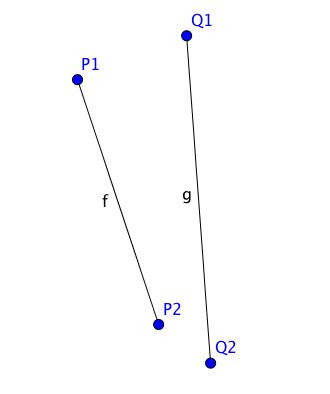
\includegraphics{img/segments_basic.png}
    \caption{Řezy v rovině $ \rho $}
  \centering
  \label{fig:segments_basic}
\end{figure}

Nyní už ale k samotnému posunu. Prvně zajistíme, aby oba dva vrcholy ležely ve
správné polorovině. K tomu nám poslouží vektory
\begin{align*}
    v_1 = Q_1 - V^{center} \qquad\text{a}\qquad v_2 = Q_2 - V^{center}.
\end{align*}

Díky podmínce \ref{cond:halfspace} nastane vždy nejvýše jedna
ze dvou možností. Buďto $ {\langle V^{normal}, v_1\rangle < 0 }$ a je potřeba
přesunout vrchol $ Q_1 $. Posun provedeme ve směru normály $ V^{normal} $ položením
$ Q_1 = P_1 + \epsilon V^{normal} $, kde $ \epsilon $ může být opět libovolné
kladné číslo menší než $ \delta $, nicméně v rámci alespoň částečného zachování
zamýšleného směrování tunelu je vhodné jej volit co nejmenší. Experimentálně
jsme ověřili, že vhodnou volbou je například $ \epsilon = \frac{\delta}{100} $.

V případě, že $ \langle V^{normal}, v_2\rangle < 0 $, postupujeme zcela analogicky
pro vrcholy $ P_2 $, $ Q_2 $. Nakonec ještě v případě nutnosti přeznačením
zajistíme správnou korespondenci, neboť ta by se mohla v některých patologických
případech našimi úpravami porušit. Tím jsou vyřešeny podmínky
(\ref{cond:not_intersecting}) a (\ref{cond:going_forward}).

Teď když máme vrcholy na správné straně, můžeme provést úpravy, které zajistí,
že nejsou příliš daleko od sebe. Prakticky to znamená pro obě dvojice
korespondujících vrcholů spočítat $ w_i = Q_i - P_i $ a pokud platí
$ \norm{w_i} > \delta $ provedeme posun
$ Q_i = P_i + \tilde{\epsilon} \frac{w_i}{\norm{w_i}} $, kde
$ 0 < \tilde{\epsilon} < \delta $.

Experimentálně jsme ověřili, že vhodnou volbou pro $ \tilde{\epsilon} $ je
$ \tilde{\epsilon} = \frac{95}{100} \delta$. Vzdálenost takto generovaných řezů
byla dostatečně blízko k $ \delta $, ale zároveň byl počet rekurzivních zanoření
minimální (nejvýše 2) a dopad na celkový výkon algoritmu nebyl vůbec měřitelný
(rekurzivní volání se realizuje na řádku \ref{shiftDisk:recursion} a jeho důvody
ještě rozebereme). Proč za epsilon nezvolit přímo $ \delta $ bude zřejmé z
pozdějšího textu.

Z výsledných bodů zrekonstruujeme řez, jehož střed je určen vrcholy
$ Q_1 $, $ Q_2 $, a normála $ \vec{n} $ bude vektor ležící v rovině $ \rho $
kolmý na vektor $ \overrightarrow{Q_1 Q_2} $, který orientujeme tak, že bude platit
$ \langle V^{normal}, \vec{n} \rangle \geq 0 $, tedy vyžadujeme souhlasnou
orientaci, jakou má předchozí řez. Nakonec zavoláme funkci
$ \operatorname{fitDiskTunnel} $, která zajistí správně zvolený poloměr.
Uvedený postup shrnuje pseudokód č. \ref{alg:shiftDisk}:


\begin{algorithm}
\caption{Posun řezu}
\label{alg:shiftDisk}
\begin{algorithmic}[1]

\Function{shiftDisk}{$ V, W$}
    \State $ P_1, P_2, Q_1, Q_2 \gets $ Proper vertex correspondence
    \State $ \vec{v_1} \gets Q_1 - V^{center} $
    \State $ \vec{v_2} \gets Q_2 - V^{center} $
    \Statex

    \If {$ \langle V^{normal}, \vec{v_1} \rangle < 0 $}
        \State $ Q_1 \gets P_1 + \epsilon V^{normal} $
    \ElsIf {$ \langle V^{normal}, \vec{v_2} \rangle < 0 $}
        \State $ Q_2 \gets P_2 + \epsilon V^{normal} $
    \EndIf
    \State $ P_1, P_2, Q_1, Q_2 \gets $ Proper vertex correspondence
    \Statex

    \State $ \vec{w_1} \gets Q_1 - P_1 $
    \If {$ \norm{w_1} > \delta $}
        $ Q_1 \gets P_1 + \tilde{\epsilon} \frac{\vec{v_1}}{\norm{w_1}} $ \label{shiftDisk:correction1}
    \EndIf

    \State $ \vec{w_2} \gets Q_2 - P_2 $
    \If {$ \norm{w_2} > \delta $}
        $ Q_2 \gets P_2 + \tilde{\epsilon} \frac{\vec{v_2}}{\norm{w_2}} $ \label{shiftDisk:correction2}
    \EndIf
    \Statex

    \State $ Z \gets $ Construct disk from $ Q_1$, $Q_2$ perpendicular to $ \rho $
    \State $ W \gets \operatorname{fitDiskTunnel}(Z^{normal}, Z^{center}) $ \label{shiftDisk:fit}
    \Statex

    \If {$ \dst(V, W) > \delta \vee \neg \operatorname{isFollower}(V, W)$ }
        \State \Return $ \operatorname{shiftDisk}(V, W) $ \label{shiftDisk:recursion}
    \Else
        \State \Return $ W $
    \EndIf

\EndFunction

\end{algorithmic}
\end{algorithm}

Poslední úprava na řádku \ref{shiftDisk:fit} by ještě v některých případech mohla
porušit podmínku na vzdálenost. Kvůli tomu zvolíme na řádcích
\ref{shiftDisk:correction1} a \ref{shiftDisk:correction2} posun o něco
menší než je $ \delta $. Pokud nový řez bude i tak porušovat podmínku (\ref{cond:distance}),
případně podmínky (\ref{cond:not_intersecting}) a (\ref{cond:going_forward})
(jejíž splnění kontroluje funkce $ \operatorname{isFollower} $),
aplikujeme celý postup rekurzivním voláním na řádku \ref{shiftDisk:recursion} znovu.

Díky tomu algoritmus pro každý vstup vrátí správný výsledek, pokud zastaví.
Jak je to tedy s konečnosti výpočtu? Algoritmus $\operatorname{fitDiskTunnel} $
nemění normálový vektor řezu a proto
rovina $ \rho $ zůstane během rekurze stále stejná. Díky tomu jistě úsečku
$ \widetilde{W} $ při každém rekurzivním zanoření posuneme o kousek blíže k
$ \widetilde{V} $. To společně se spojitostí a konečnými rozměry tunelu zajistí,
že se po konečném počtu kroků dostaneme do vzdálenosti menší než $ \delta $.

Zevrubným testováním jsme zjistili, že problém může nastat ve chvíli, kdy
z důvodu prudké změny poloměru nebo směru tunelu nemůžeme pokračovat vpřed, aniž
bychom porušili některou z našich podmínek kladených na posloupnost řezů.
Tuto situaci dobře demonstruje obrázek \ref{fig:sharp_curve}. V této situaci
téměř jakékoliv posunutí vpřed vyústí v prudké změny poloměru minimální kružnice
obepínající tunel a algoritmus v tomto případě selže. V tuto chvíli se buďto
můžeme spustit nějakou formu backtrackingu nebo se pokusíme pravděpodobnost
této situace minimalizovat, což v našem případě bude znamenat, že zvolíme v případě
detekce potenciálně velmi prudkého ohybu jinou strategii a funkci
$ \operatorname{shiftDisk} $ spustíme jen když toto nebezpečí nebude hrozit.

\begin{figure}[ht]
    \centering
    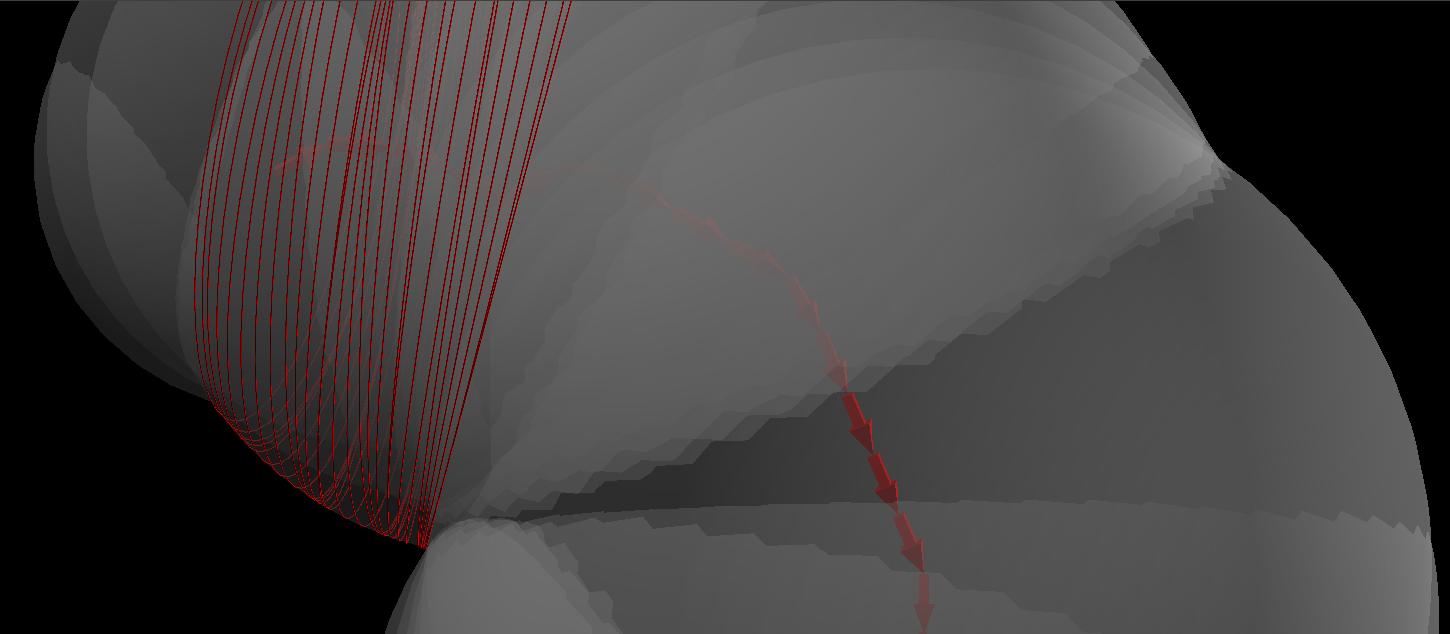
\includegraphics[width=\textwidth]{img/sharp_curve.png}
    \caption{Prudké zatočení se změnou poloměru}
  \centering
  \label{fig:sharp_curve}
\end{figure}





\section{Funkce shiftSharpTurn} \label{subsec:shift_sharp_turn}
Předchozí popsanou funkci doplňuje procedura $ \operatorname{shiftSharpTurn} $.
Jejím účelem je implementovat prostřednictvím aktuálního řezu maximální možné
zatočení při zachování všech podmínek.

Funkce v případě blížící se prudké
zatáčky načte poslední umístěný řez a posune jej vpřed o $ \Delta $ ve směru
jeho normály. To se realizuje na řádcích \ref{alg:shift_by_delta} a
\ref{alg:same_normal} v hlavním algoritmu. Na takto posunutý řez aplikujeme
funkci $ \operatorname{fitDiskTunnel} $. Tímto způsobem získáme docela dobrou
představu o tom, co se s tunelem v nejbližší době bude dít, na základě čehož
můžeme implementovat případné korekce a orientovat nový řez směrem, kterým
tunel zatáčí.

Na vstupu funkce $ \operatorname{shiftSharpTurn} $ tedy budeme mít předchozí
umístěný řez, resp. aktuálně umisťovaný řez s výše uvedenými vlastnostmi,
které si označíme $ V $,
resp. $ W $. Stejně jako u předešlé funkce budeme chtít veškeré výpočty provádět
v projekci do nějaké roviny. Označme si tuto rovinu $ \rho $.
V tomto případě však budou mít oba řezy stejný
normálový vektor, což nám dává možnost volby. Zamysleme se tedy nad tím,
jak zvolit druhý vektor projekční roviny. Obrázek \ref{fig:sharp_curve_lookahead}
dobře ilustruje, jak taková situace může vypadat. Z tohoto bočního pohledu je
zřejmé, že bychom měli řez posunout v maximální možné míře dopředu v horní části
tunelu a zafixovat pohyb řezu v jeho dolní části, jinak bychom se brzy dostali
právě do vyobrazené situace. Pro srovnání uvádíme pohled z jiného úhlu na stejnou
situaci v podobě obrázku \ref{fig:sharp_curve_lookahead_from_up}.

\begin{figure}[ht]
\centering1
\begin{minipage}{.6\textwidth}
  \centering
        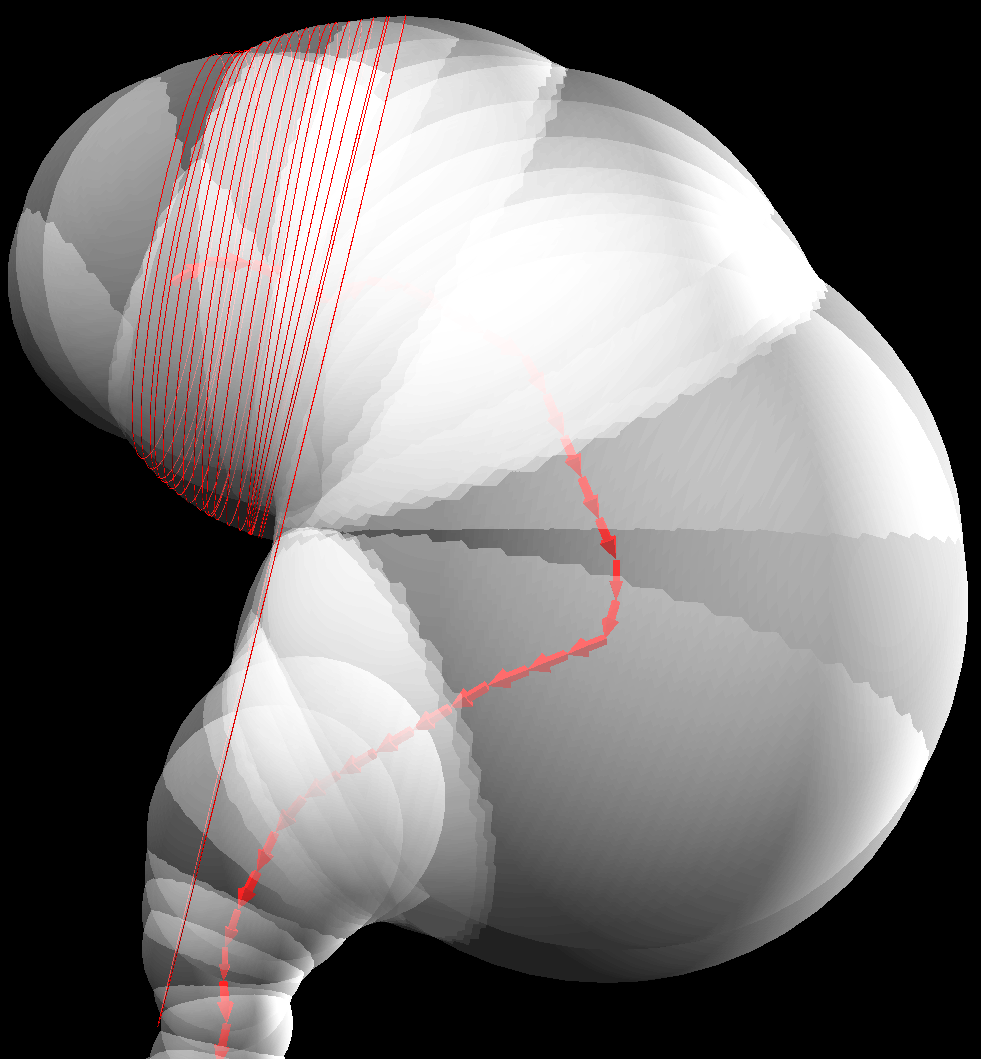
\includegraphics[width=75mm]{img/sharp_curve_lookahead.png}
        \caption{Prudké zatočení, pohled z boku}
    \centering
    \label{fig:sharp_curve_lookahead}
\end{minipage}%
\begin{minipage}{.4\textwidth}
    \centering
        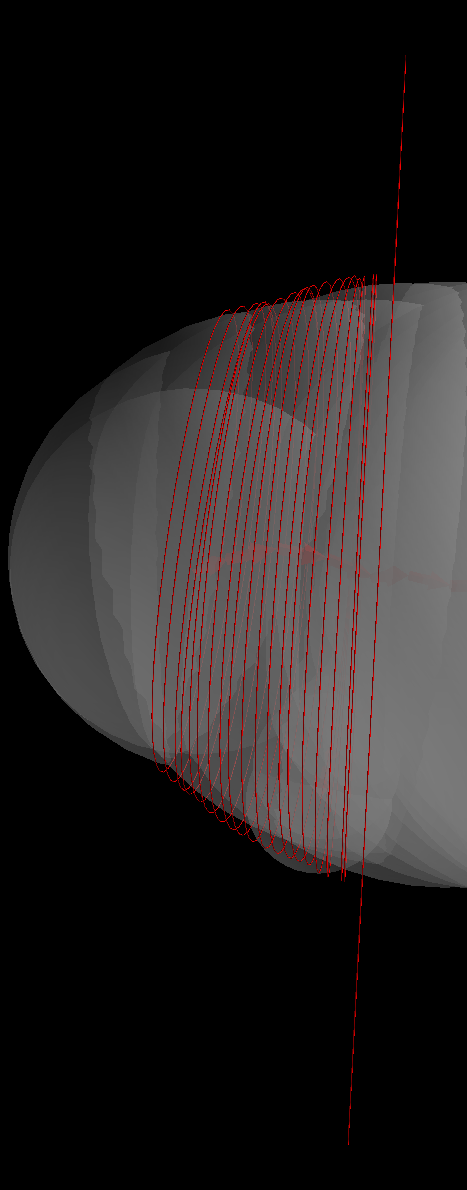
\includegraphics[width=40mm]{img/sharp_curve_lookahead_up.png}
        \caption{Prudké zatočení, pohled shora}
    \centering
    \label{fig:sharp_curve_lookahead_from_up}
\end{minipage}
\end{figure}

Je zřejmé, že na výběru druhého vektoru projekční roviny skutečně záleží, neboť
například pohled shora nedává žádnou indicii o tom, jakým způsobem bychom
se měli zachovat. Prakticky ale stačí vzít vektor, který je
určen středy našich řezů, tedy vektor $ {v = W^{center} - V^{center} }$. Ze všech
přípustných rovin pak takto vzniklá rovina bude maximalizovat vzdálenost mezi
středy úseček vzniklých projekcí řezů do $ \rho $. Také díky tomu, že
výsledná rovina bude obsahovat oba středy našich řezů, dostaneme v projekční
rovině nedeformované úsečky o maximálních délkách – jejich průměr bude stejný
jako průměr promítaných řezů.

Teoreticky by se nám ještě mohlo stát, že by takto vzniklý vektor a normálový
vektor $ V^{normal} $ byly lineárně závislé. V taktovém případě k žádnému
zatočení zřejmě nedochází. Popisovaný algoritmus bude i tak fungovat,
a to pro libovolnou volbu vektoru lineárně nezávislého na $ V^{normal} $.

Když máme k dispozici projekční rovinu, můžeme podobně jako v případě
procedury $ \operatorname{shiftDisk} $ najít korespondující
vrcholy $ P_1, P_2 $, resp. $ Q_1, Q_2 $. Nyní je potřeba rozlišit dva případy.

Pokud $ W^{radius} \geq V^{radius} $, pak pomocí vrcholů úseček zjistíme, která
dvojice korespondujících vrcholů je od sebe dál, a tu pak ztotožníme. V případě
druhé dvojice umístíme vrchol $Q_i $ do vzdálenosti menší než $\delta$ od vrcholu
$ P_i $. Tuto situaci můžeme vidět na obrázku \ref{fig:sharp_curve_lookahead}.

Jestliže platí $ V^{radius} > W^{radius} $, ztotožníme naopak dvojici vrcholů,
která má k sobě blíže a do vzdálenosti menší než $\delta$ posuneme druhou dvojici.
Ilustrativní příklad je znázorněn na obrázku \ref{fig:sharp_curve_lookahead_decrease}.

\begin{figure}[ht]
    \centering
    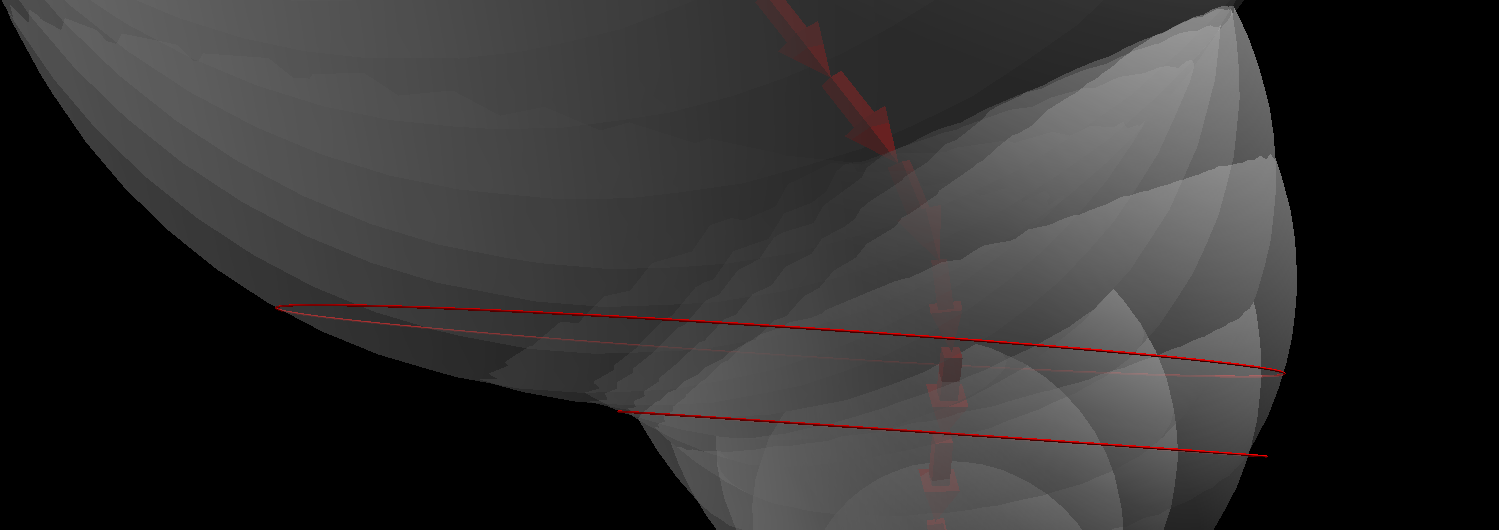
\includegraphics[width=\textwidth]{img/sharp_curve_lookahead_decrease.png}
    \caption{Prudké zmenšení poloměru}
  \centering
  \label{fig:sharp_curve_lookahead_decrease}
\end{figure}

Intuitivně toto rozdělení můžeme chápat tak, že pokud průměr tunelu v daném směru
neklesá, pak naše počínání v místě ostrého zatočení zvětší úhel, který v daném
místě svírá řez se stěnou tunelu (v rovině $ \rho $). Abychom tento úhel zvětšili
i v případě poklesu poloměru, musíme naopak ztotožnit body, které k sobě mají
blíže.

Nakonec na základě takto posunutých vrcholů vygenerujeme nový řez. Uvedený
postup je zachycen pseudokódem č. \ref{alg:shiftSharpTurn}.

\begin{algorithm}
\caption{Posun řezu pro ostré zatáčky}
\label{alg:shiftSharpTurn}
\begin{algorithmic}[1]

\Function{shiftSharpTurn}{$ V, W$}
    \State $ \rho \gets $ Projection plane described in text
    \State $ P_1, P_2, Q_1, Q_2 \gets $ Proper vertex correspondence
    \State $ \vec{v_1} \gets Q_1 - P_1 $
    \State $ \vec{v_2} \gets Q_2 - P_2 $
    \State $ d_1 \gets \norm{\vec{v_1}} $
    \State $ d_2 \gets \norm{\vec{v_2}} $

    \Statex
    \If {$ V^{radius} > W^{radius} $}
        \State $ \operatorname{\mathbf{Swap}}(d_1, d_2) $
    \EndIf

    \Statex
    \If {$ d_1 > d_2 $} \label{shiftSharpTurn:begin_ifs}
        \State $ Q_1 \gets P_1$
    \Else
        \State $ Q_1 \gets P_1 + \operatorname{norm}(\vec{v_1}) * \delta * \frac{95}{100} $
    \EndIf
    \If {$ d_1 < d_2 $}
        \State $ Q_2 \gets P_2$
    \Else
        \State $ Q_2 \gets P_2 + \operatorname{norm}(\vec{v_2}) * \delta * \frac{95}{100} $ \label{shiftSharpTurn:end_ifs}
    \EndIf

    \Statex
    \State $ Z \gets $ Construct disk from $ Q_1$, $Q_2$ perpendicular to $ \rho $
    \State $ W \gets \operatorname{fitDiskTunnel}(Z^{normal}, Z^{center}) $
    \Statex

    \If {$ \dst(V, W) > \delta \vee \neg \operatorname{isFollower}(V, W)$ }
        \State \Return $ \operatorname{shiftDisk}(V, W) $ \label{shiftSharpTurn:shift_disk}
    \Else
        \State \Return $ W $
    \EndIf

\EndFunction

\end{algorithmic}
\end{algorithm}

Rozeberme si ještě některé detaily uvedené procedury. Na řádcích
\ref{shiftSharpTurn:begin_ifs} až \ref{shiftSharpTurn:end_ifs} můžeme vidět, že
algoritmus každý z vrcholů posune buďto identicky na korespondující vrchol
předchozího řezu nebo do vzdálenosti o něco menší než $ \delta $. Posun přímo
o $ \delta $ opět záměrně nevolíme, abychom předešli zbytečným opravám. Zde si
také můžeme všimnout, že pokud máme na vstupu řezy, jejichž spojnice středů
se dá vyjádřit jako lineární kombinace jejich normál, pak zřejmě bude platit
$ \norm{\vec{v_1}} = \norm{\vec{v_2}} $. Tunel se tedy v tomto místě
pravděpodobně ubírá přímo rovně. V souladu s tímto faktem se v obou případech
větvení vydáme druhou větví a oba vrcholy umístíme do stejné vzdálenosti, čímž
zajistíme přímý pohyb tunelem.

Stejně jako v případě funkce $ \operatorname{shiftDisk} $ musíme nakonec
zkontrolovat splnění našich podmínek ze stejných důvodů jako u funkce
\ref{alg:shiftDisk} a v případě jejich porušení voláme ještě
na řádku \ref{shiftSharpTurn:shift_disk} funkci $ \operatorname{shiftDisk} $,
která umístění řezu dokončí.





\section{Funkce isSharpTurn} \label{subsec:is_sharp_turn}
To, zda použijeme funkci $ \operatorname{shiftDisk} $ nebo radikálnější
$ \operatorname{shiftSharpTurn} $, rozhodujeme na základě návratové hodnoty
funkce $ \operatorname{isSharpTurn} $. Ta podobně jako v těle hlavního
algoritmu \ref{alg:digTunnel} posune poslední umístěný řez o konstantu
$ \Delta $ ve směru jeho normály. Sečnou rovinu zkonstruujeme stejně jako v
případě funkce $ \operatorname{shiftSharpTurn} $ a v ní najdeme korespondující
vrcholy $ P_1$, $P_2$, $Q_1$ a $ Q_2 $. Následně zjistíme procentuální rozdíl
mezi vzdálenostmi vrcholů. Ostrou zatáčku pak implementujeme ve chvíli, kdy se
vzdálenosti liší o více než 35 \%. Tato hranice nepoměru se nám v praxi osvědčila
velmi dobře. Výpočet je zachycen pseudokódem č. \ref{alg:isSharpTurn}.

\begin{algorithm}
\caption{Detekce ostré zatáčky}
\label{alg:isSharpTurn}
\begin{algorithmic}[1]

\Function{isSharpTurn}{$ V, W$}
    \State $ \rho \gets $ Projection plane described in chapter \ref{subsec:shift_sharp_turn}
    \State $ P_1, P_2, Q_1, Q_2 \gets $ Proper vertex correspondence
    \State $ \vec{v_1} \gets Q_1 - P_1 $
    \State $ \vec{v_2} \gets Q_2 - P_2 $
    \State \Return $ \frac{\left| \norm{\vec{v_1}} - \norm{\vec{v_2}} \right|}
                          {\frac{\norm{\vec{v_1}} + \norm{\vec{v_2}}}{2}} > 0.35$
\EndFunction

\end{algorithmic}
\end{algorithm}





\section{Směrování tunelu} \label{subsec:tunnel_dir}
Jak už jsme dříve rozebírali, pro správnou funkci algoritmu je nezbytné, abychom
v libovolném místě tunelu měli k dispozici informaci o tom, kterým směrem bychom
se měli dále pohybovat. Pro potřeby formálního popisu potřebujeme
po částech konstantní křivku $ \gamma(t) \colon [0, l] \to \Rbb^3$
parametrizovanou obloukem, která bude
určena posloupností bodů ležících uvnitř tunelu o celkové délce $ l $. Tyto body
budeme značit $ C_i $ a pro začátek je definujeme jakožto středy koulí našeho tunelu:
$ \{C_i = S_i^{center}\}_{i=0}^{n} $.

Podél křivky $ \gamma(t) $ se můžeme tunelem pohybovat a přirozeně bychom pro
směrování našeho algoritmu v bodě $ t_0 $ chtěli použít směr pohybu – derivaci
$ \frac{d\gamma}{dt}(t_0) $. Narazíme však na to, že pro $ t_0 $ taková, že
$ \gamma(t_0) = C_i $ pro nějaké $ 0 < i < n $ derivace neexistuje. To můžeme
napravit tak, že namísto $ \frac{d\gamma}{dt}(t_0) $ budeme definovat vektorové
pole $ \Omega(t) \colon [0, l] \to \Rbb^3 $. Pro libovolné $ t_0 \in [0, l] $
můžeme najít body $ C_i $ a $ C_{i + 1} $ na křivce $ \gamma $, mezi kterými
se nachází bod $ \gamma(t_0) $. Vektorové pole v bodě $ t_0 $ pak definujeme
jakožto

\begin{align}
    \Omega(t_0) =
            (1 - \lambda) \operatorname{norm}(C_{i + 1} - C_i)
            +
            \lambda \operatorname{norm}(C_{i + 2} - C_{i + 1})
        ,
\end{align}
kde
\begin{align}
    \lambda = \frac{\norm{\gamma(t_0) - C_i}}{\norm{C_{i + 1} - C_i}}
\end{align}
pokud $ i + 2 \leq n $, jinak
\begin{align}
    \Omega(t_0) = \operatorname{norm}(C_{i + 1} - C_i).
\end{align}

Prakticky se jedná o jednoduchý vážený průměr, který postupně mezi jednotlivými středy
$ C_i $ spojitě transformuje jeden směrový vektor na druhý.

Jak jsme ale mohli vidět na obrázku \ref{fig:naive_cuts}, použití takto definovaných
směrových vektorů jakožto normál řezů vyústí v silně volatilní posloupnost,
a tak je potřeba vektorové pole $ \Omega $ ještě dále vyhladit.

Uvažme tedy opět libovolný bod $ t_0 \in [0, l] $ pro který chceme získat vektor,
který co nejlépe vystihuje směr tunelu v daném bodě. Nechceme pro tyto účely použít
přímo vektorové pole $ \Omega $, protože to by mohlo být příliš volatilní
a nemuselo by dobře reflektovat globální směr tunelu. Namísto toho můžeme spočítat,
jak se v průměru chová $ \Omega $ na okolí bodu $ t_0 $. Formálně budeme
definovat nové vektorové pole $ \Phi \colon [0, l] \to \Rbb^3 $,

\begin{align}
    \Phi(t_0) = \int_{t_1 = \max\{t_0 - \Delta, 0\}}^{t_2 = \min\{t_0 + \Delta, l\}}
        \Omega(t) (\Delta - \left| t_0 - t \right| )^2 dt.
\end{align}

Zjednodušeně řečeno, funkce $ \Phi $ realizuje součet vektorů vektorového pole,
$ \Omega $ jejichž váha kvadraticky klesá se zvyšující se vzdáleností od bodu
$ t_0 $, a to až do maximální vzdálenosti $ \Delta $. (V praxi se nám osvědčilo
nastavení $ \Delta = 5 Å $, kde Å je značkou pro jednotku délky angstrom, běžně
používanou v chemii. Hodnota jednoho angstromu je rovna 0.1 nm.)

Uvedený integrál budeme v průběhu výpočtu potřebovat prakticky vyhodnocovat,
musíme jej proto vypočítat. Pro začátek předpokládejme, že křivka $ \gamma $ na
intervalu $ [t_1, t_2] $ prochází alespoň jedním bodem $ C_i $. To znamená, že
existuje neprázdná množina středů $ {P = \{C_k, \dots, C_{k + m} \} }$ taková, že
$ C \in P \Rightarrow \gamma^{-1}(C) \in [t_1, t_2]$. Označme
$ f(t) = \Omega(t) (\Delta - \left| t_0 - t \right| )^2 $. Potom $ \Phi $ můžeme zapsat
následujícím způsobem:

\begin{align} \label{eq:integral_sum}
    \Phi(t_0) = \int_{t_1}^{\gamma^{-1}(C_k)} f(t) dt
        + \sum_{j=0}^{m - 1} \int_{\gamma^{-1}(C_{k + j})}^{\gamma^{-1}(C_{k + j + 1})} f(t) dt
        + \int_{\gamma^{-1}(C_{k + m})}^{t_2} f(t) dt
\end{align}

Sčítance uprostřed uvedeného výrazu odpovídají integraci po úsečce vždy mezi
dvěma po sobě jdoucími středy $ C_i $, $C_{i+1} $. Toho využijeme a nejprve ukážeme,
jak počítat integrály tohoto typu. Označme $\alpha = \norm{C_{i + 1} - C_i}$.
Díky tomu, že je křivka $ \gamma $ parametrizovaná
obloukem, dostaneme substitucí
$ s(t) = \frac{t - \gamma^{-1}(C_i)}{\alpha} $ vztah

\begin{align*}
    \int_{\gamma^{-1}(C_{i})}^{\gamma^{-1}(C_{i + 1})} f(t) dt
    &= \bigg\rvert
        ^{s(t) = \frac{t - \gamma^{-1}(C_i)}{\alpha}}
        _{s'(t) = \alpha^{-1}} \bigg\lvert \\
    &= \int_{0}^{1}
        \frac{\widehat{\Omega}(s)
            \left[\Delta - \left| t_0 - (s \alpha + \gamma^{-1}(C_i)) \right| \right]^2}
        {\alpha} ds
    = (*),
\end{align*}
přičemž
\begin{align*}
    \widehat{\Omega}(s) = (1 - s) \operatorname{norm}(C_{i + 1} - C_i)
            + s \operatorname{norm}(C_{i + 2} - C_{i + 1}).
\end{align*}
To proto, že $ \lambda = s(t) $, což platí opět díky tomu, že $ \gamma $ je
parametrizovaná obloukem.

Abychom byli schopni integrál skutečně dopočítat, potřebujeme se zbavit absolutní
hodnoty. Předpokládejme proto, že $ \gamma^{-1}(C_{i + 1}) \leq t_0$ díky čemuž

\begin{align}
    (*) &= \int_{0}^{1}
        \frac{\widehat{\Omega}(s)
            \left[\Delta - (t_0 - (s \alpha + \gamma^{-1}(C_i)) ) \right]^2}
        {\alpha}
         ds \\
    &= \frac{1}{12} \left(
        \frac{6 d^2 (v_1+v_2 )}{\alpha}
        + 4 d (v_1+2 v_2 )
        + \alpha (v_1+3 v_2 ) \right), \label{eq:result_1}
\end{align}
kde $ d = \Delta - t_0 + \gamma^{-1}(C_i) $,
$ v_1 = \operatorname{norm}(C_{i + 1} - C_i) $ a
$ v_2 = \operatorname{norm}(C_{i + 2} - C_{i + 1})$.

Podobně za předpokladu že $ \gamma^{-1}(C_i) \geq t_0$ dostáváme
\begin{align}
    (*) &= \int_{0}^{1}
        \frac{\widehat{\Omega}(s)
            \left[\Delta + (t_0 - (s \alpha + \gamma^{-1}(C_i)) ) \right]^2}
        {\alpha}
         ds \\
    &= \frac{1}{12} \left(
        \frac{6 d^2 (v_1+v_2 )}{\alpha}
        - 4 d (v_1+2 v_2 )
        + \alpha (v_1+3 v_2 ) \right), \label{eq:result_2}
\end{align}
přičemž $ d = \Delta + t_0 - \gamma^{-1}(C_i) $.

Tímto způsobem jsme schopni vypočítat hodnotu integrálu mezi dvěma po sobě jdoucími
body $ C_i $ a $ C_{i + 1} $. Kvůli odstranění absolutní hodnoty jsme se ale
museli omezit na úsečky, na kterých neleží bod $ \gamma(t_0) $. Integrál, jehož
integrační interval obsahuje $ t_0 $, rozdělíme na součet dvou
integrálů

\begin{align*}
    \int_{a}^{b} f(t) dt = \int_{a}^{t_0} f(t) dt + \int_{t_0}^{b} f(t) dt.
\end{align*}

Tyto dva integrály společně s krajními integrály v součtu (\ref{eq:integral_sum})
jsou z definice posloupnosti $ P $ integrály na intervalu, na kterém je křivka
$ \gamma(t) $ konstantní. Označme si meze takovéhoto integrálu $ c $ a $ d $.
Pak ale existují vrcholy $ C_i $ a $ C_{i + 1} $ křivky $ \gamma $ takové, že
$ [c, d] \subseteq [\gamma^{-1}(C_i), \gamma^{-1}(C_{i + 1})] $. Díky tomu stačí
k výpočtu použít vzorečky (\ref{eq:result_1}) nebo (\ref{eq:result_2}), podle
toho, zda jsme před, nebo za bodem $ t_0 $, s tím, že
namísto integračního intervalu $ [0, 1] $ zvolíme interval
$ \left[ \frac{c - \gamma^{-1}(C_i)}{\gamma^{-1}(C_{i + 1}) - \gamma^{-1}(C_i)},
 \frac{d - \gamma^{-1}(C_i)}{\gamma^{-1}(C_{i + 1}) - \gamma^{-1}(C_i)} \right] $.

Pokud by $ P $ byla náhodou prázdná, budeme postupovat
analogicky podle výše uvedeného postupu. Poznamenejme, že ač je to velmi
nepravděpodobné, teoreticky by se mohlo dojít k tomu, že bychom po vypočtení
hodnoty $ \Phi(t_0) $ dostali nulový vektor. V takové situaci bychom jednoduše
namísto $ \Phi $ použili aktuální směr trajektorie tunelu v daném místě.

Doposud jsme tedy definovali křivku $ \gamma $ určenou středy koulí určujících
tunel. Podél křivky $ \gamma $ jsme definovali vektorové pole $ \Omega $, které
jsme dále ještě vyhladili pomocí integrace po křivce do podoby vektorového
pole $ \Phi $. Tento přístup sám o sobě nám dává poměrně spolehlivou informaci
o tom, jakým směrem se v daném místě tunelu orientovat. Potíž ovšem
může být ve volbě výchozí křivky $ \gamma $. Konkrétně jde o volbu řídících bodů,
které křivku určují. Některé koule tunelu mohou do jeho povrchu a celkového
tvaru přispívat jen velmi málo nebo dokonce vůbec a jiné naopak hodně, avšak na tvar
křivky $ \gamma $ mají vliv prakticky stejný. V případě některých tunelů
toto může způsobovat nemalé problémy a algoritmus pak může být směrován úplně
špatným směrem, což může vést k mnohem delšímu běhu, nižší kvalitě řezů, nebo
úplnému selhání algoritmu. Abychom tyto obtíže překonali, musíme volit
řídící body křivky $ \gamma $ tak, aby co nejlépe vystihovaly střed objemu
tunelu v jeho zadané části. Prakticky budeme pro každý střed $ C_i $ hledat řez,
ve kterém tento bod leží a který má zároveň co nejmenší poloměr. Jak takový
řez najít je obsahem následující podkapitoly.






\section{Hledání minimálního řezu} \label{subsec:min_cut}
Úlohu nalezení minimálního řezu můžeme formulovat jako úlohu nalezení minima
funkce $ \operatorname{fitDiskTunnel} $ (minimum bráno podle průměru umístěného řezu)
nad množinou vektorů daných jednotkovou sférou (ve skutečnosti stačí brát
jen polovinu – hemisféru – díky symetrii).

Na tento problém jsme se pokusili aplikovat řadu metod implementovaných v Python
knihovně SciPy, namátkou uveďme například simulované žíhání, Nelder-Meadovu metodu
nebo Broyden-Fletcher-Goldfarb-Shannův algoritmus. Vedle těchto metod jsme zároveň
ještě implementovali vlastní, poměrně naivní prohledávání. Výsledky byly
překvapivé. Obecné metody byly zpravidla schopny globální minimum mnohem přesněji
lokalizovat a obvykle nacházely řešení, které bylo oproti našemu vlastnímu
algoritmu o jednotky procent lepší, avšak v případě některých komplikovanějších
tunelů se stávalo, že uvázly v lokálním minimu, které se od globálního lišilo
o desítky procent, kdežto náš naivní přístup tímto způsobem neselhal ani jednou.
Je ale nutno podotknout, že uvedené obecné metody by potenciálně mohly fungovat
dobře, pokud by autor při implementaci věnoval více času ladění jejich parametrů,
případně adaptaci vstupní úlohy, aby lépe odpovídala typickým úlohám, které tyto
algoritmy řeší dobře.

V našem případě jsme ovšem dali přednost naší naivní metodě, která
fungovala velmi spolehlivě s dostatečnou přesností. Zmiňovaný přístup popisuje
pseudokód č. \ref{alg:findMinimalDisk}.


\begin{algorithm}
\caption{Algoritmus pro hledání orientace, ve které bude mít řez minimální poloměr}
\label{alg:findMinimalDisk}
\begin{algorithmic}[1]


\Function{findMinimalDisk}{$ P, \vec{n}$}
    \State $ V  \gets \operatorname{fitDiskTunnel}(\vec{n}, P) $
    \For{$ i = 0, \dots, 4 $}
        \State $ \theta \gets \frac{\pi / 3}{4^i} $ \label{alg:findMinimalDisk:dec_angle}
        \State $ found\_better \gets $ True
        \While {$found\_better$}
            \State $ found\_better \gets $ False
            \State $ \vec{v} \gets V^{normal} $
            \For{$ \varphi \in \{ k \frac{i + 1}{10} \mid k \frac{i + 1}{10} < 2 \pi, k \in \Nbb \}$} \label{alg:findMinimalDisk:inner_for}
                \State $ \vec{w} \gets$ Vector $\vec{v} $ rotated by $ \theta $ and $\varphi $ \label{alg:findMinimalDisk:rotate}
                \State $ W \gets \operatorname{fitDiskTunnel}(\vec{w}, P) $
                \If{$ W^{radius} < V^{radius} \wedge $ Tunnel trajectory threads through $ W $}  \label{alg:findMinimalDisk:if}
                    \State $ V \gets W $
                    \State $ found\_better \gets $ True
                \EndIf
            \EndFor
        \EndWhile
    \EndFor
    \State \Return $V$
\EndFunction

\end{algorithmic}
\end{algorithm}

Uvedený algoritmus funguje tak, že pro aktuálně nejlepší nalezený řez vždy nejprve
zkusí prohledat kruhové okolí kolem jeho normály, na kterém buďto najde normálu,
pro kterou dostaneme řez o menším poloměru, nebo nenajde lepší řez a v tu chvíli
na řádku \ref{alg:findMinimalDisk:dec_angle} zmenšíme úhel odklonu $ \theta $
od aktuální normály a celý proces zopakujeme.
Vnější cyklus uvedeného algoritmu tedy ovlivňuje, jak široké okolí budeme ve vnitřních
cyklech prohledávat a s jakým krokem budeme na řádku \ref{alg:findMinimalDisk:inner_for}
zvětšovat úhel $\varphi $. Rotací na řádku \ref{alg:findMinimalDisk:rotate} rozumíme to,
že vektor $\vec{v} $ nejprve odkloníme o úhel $ \theta $ a následně jej rotujeme
kolem osy určené původním $\vec{v} $. Tento proces je znázorněn na obrázku
\ref{fig:vector_rotate} s tím, že osa z v našem případě odpovídá směru vektoru
$\vec{v} $.

\begin{figure}[ht]
    \centering
    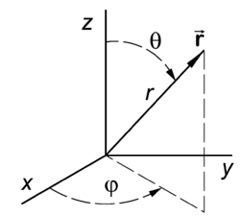
\includegraphics[width=40mm]{img/vector_rotate.jpg}
    \caption{Rotace vektoru}
  \centering
  \label{fig:vector_rotate}
\end{figure}

Posledním detailem tohoto algoritmu je druhá podmínka na řádku \ref{alg:findMinimalDisk:if},
která omezuje množinu přípustných řezů a je obecně potřeba, ať už použijeme
jakoukoliv optimalizační metodu. V podstatě touto podmínkou zajišťujeme, že daný řez
bude skutečně řezem, konkrétně že bude dělit tunel na dvě části. Teoreticky by se nám
totiž mohlo stát, že bychom našli minimální řez, který by tunel řezal jen bokem.
Tuto situaci můžeme vidět na obrázku \ref{fig:side_cut}.

\begin{figure}[ht]
    \centering
    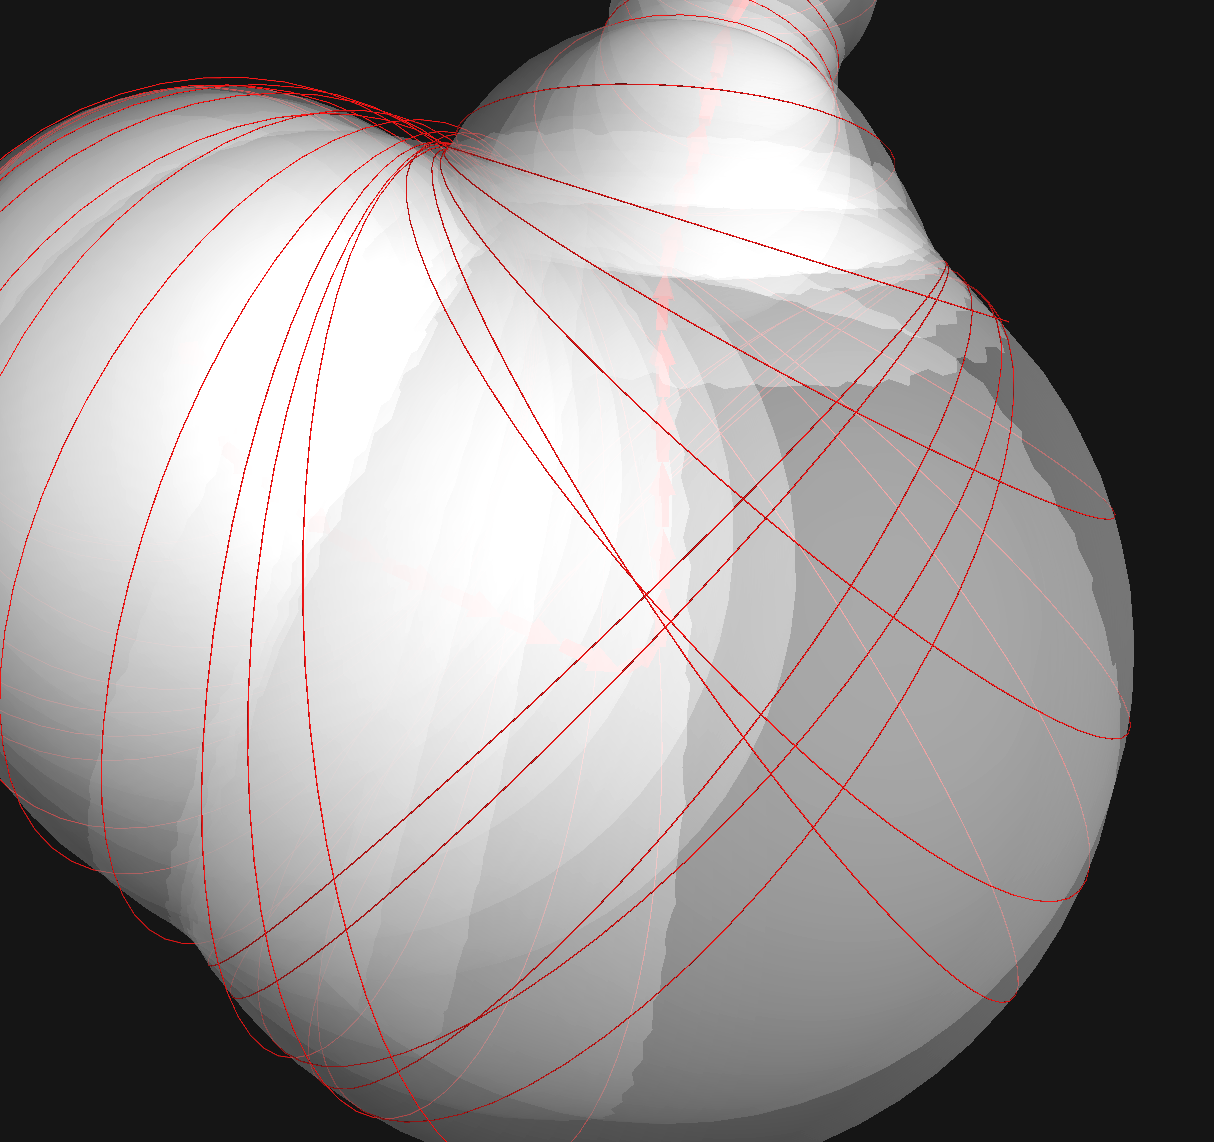
\includegraphics[width=65mm]{img/side_cut.png}
    \caption{Na obrázku můžeme vidět situaci, ve které v některých případech dojde
        k řezu bokem tunelu.}
  \centering
  \label{fig:side_cut}
\end{figure}

Prakticky algoritmus na tomto místě zjišťuje, zda trajektorie tunelu tvořená středy
koulí reálně prochází našim řezem. Vzhledem k tomu, že je trajektorie po částech
konstantní křivka, dá se toto ověření poměrně snadno implementovat.

Příklad výsledných minimálních řezů, které jsme spočítali tímto algoritmem,
můžeme vidět na obrázku \ref{fig:min_cuts}.

\begin{figure}[ht]
    \centering
    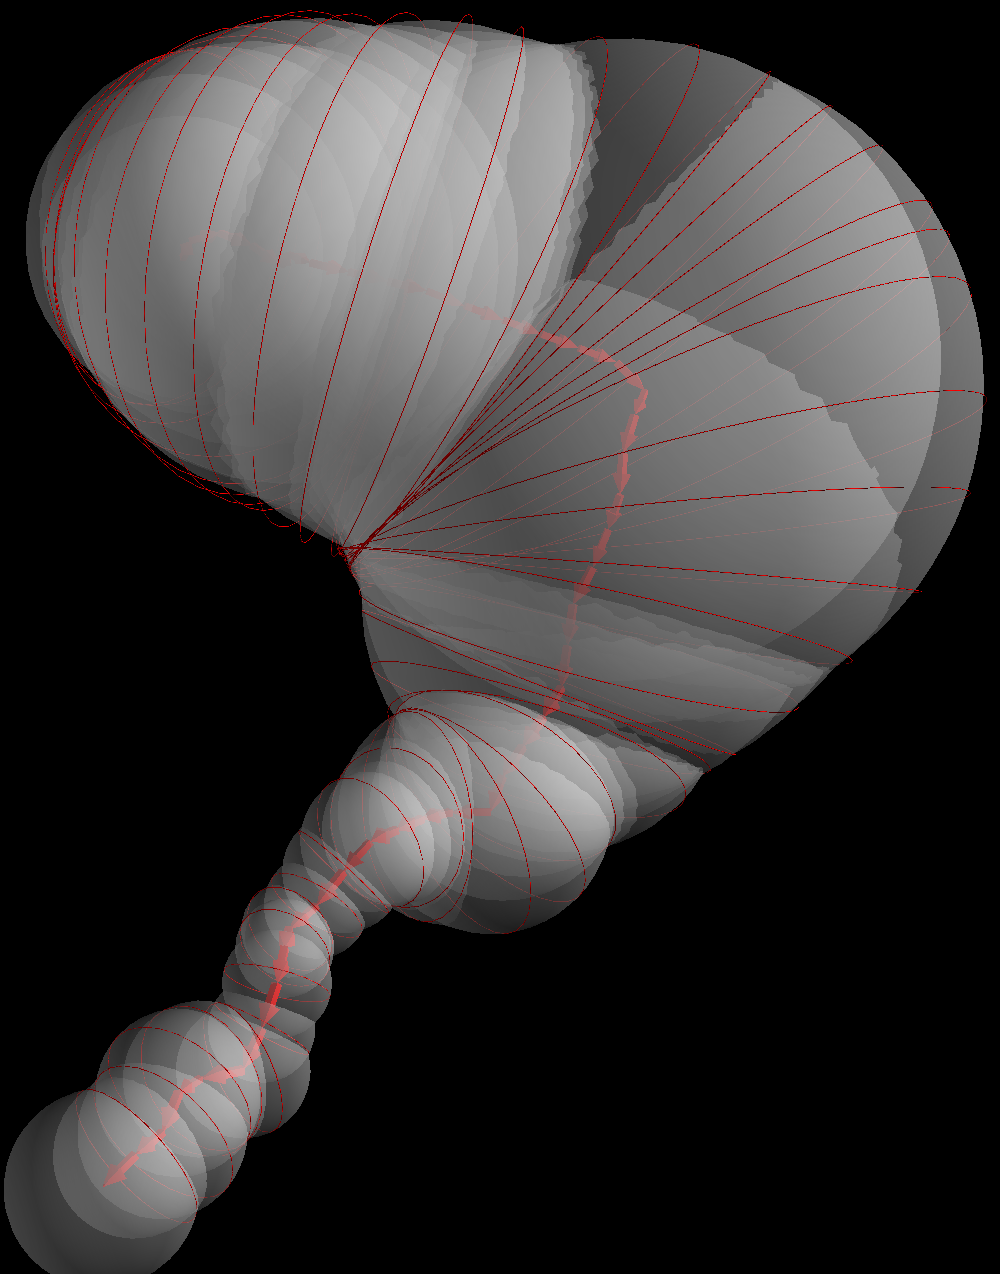
\includegraphics[width=100mm]{img/min_cuts.png}
    \caption{Minimální řezy}
  \centering
  \label{fig:min_cuts}
\end{figure}

Středy výsledných řezů nakonec vezmeme a zkonstruujeme pomocí nich křivku
$ \gamma $ z předchozí kapitoly, se kterou pak počítáme, jak již bylo popsáno.

\section{Implementace} \label{subsec:implementation}
Algoritmus pro diskretizaci tunelu byl v popsané podobě implementován v
jazyce Python. Tento jazyk jsme zvolili zejména proto, že jsme neočekávali, že
by bylo potřeba diskretizaci tunelu optimalizovat na rychlost výpočtu. V takové
situaci je Python poměrně jasná volba jednak díky množství kvalitních
knihoven jako je NumPy a SciPy a druhak pro rychlost, s jakou lze v Pythonu
implementovat prototypy. Rychlost vývoje byla velmi důležitým faktorem, neboť
jsme očekávali, že v průběhu vývoje budeme s přibývajícími poznatky často
přepisovat velké množství kódu. To se ukázalo být správným předpokladem
a ve výsledku dobrou volbou.

Algoritmus jsme implementovali konkrétně v Pythonu 2.7. Verzi 3 jsme nezvolili
zejména proto, že knihovna vPython použitá pro vizualizaci tunelu v současnosti
nejde snadno kombinovat s Pythonem 3. Nicméně v případě potřeby by přechod na
Python 3 byl velmi jednoduchou záležitostí za předpokladu odstranění knihovny
vPython, která pro samotný výpočet není nutná.

Důvodem, proč rychlost výpočtu není v tomto případě příliš důležitá, je to, že
(jak uvidíme v evaluační podkapitole \ref{subsec:evaluation}) výpočet diskretizace
včetně hledání minimálních disků z podkapitoly \ref{subsec:min_cut} trvá řádově
jednotky minut, kdežto algoritmus pro výpočet spojité trajektorie ligandu skrze
tunel může zabrat jednotky až desítky hodin výpočetního času.

Implementace je veřejně dostupná na GitHubu \cite{discretizer}.





\section{Evaluace} \label{subsec:evaluation}
Námi navržený a implementovaný algoritmus jsme vyhodnocovali spuštěním nad
množinou 152 různých tunelů v 35 různých proteinech s nastavením $ \delta = \frac{3}{10} $.
Tunely a molekuly byly převzaty z článků \cite{Enzymes} a \cite{Caver}, ve
kterých je možno
je najít pod jejich kódovým označením společně s jejich detailní vizualizací.
Vyhodnocení probíhalo na stroji se 4 jádrovým procesorem Intel(R) Core(TM) i7-4800MQ.

Validní diskretizaci se povedlo vypočítat bez dalších úprav parametrů pro všechny
tunely. Nejdelší dva tunely byly tvořeny 139, resp. 120 sférami, pro něž bylo
vygenerováno 833, resp. 588 řezů za 667, resp. 261 sekund, přičemž preprocessing
fáze zabrala 529, resp. 196 sekund paralelního výpočtu. Diskretizaci kratšího
z tunelů můžeme vidět na obrázku č. \ref{fig:1YGE} (diskretizaci delšího tunelu
neuvádíme, neboť jeho profil nebyl nijak zajímavý). Takto dlouhé tunely byly ale
spíše výjimkou a průměrná délka tunelu se pohybovala kolem 32 sfér a 162
výsledných řezů. Průměrná délka výpočtu byla 38 sekund, což vzhledem k délce
následného výpočtu spojité trajektorie považujeme za naprosto dostatečné.
Kompletní informace o vyhodnocení na každém tunelu uvádíme v apendixu A.
Pro zajímavost ještě na obrázcích \ref{fig:2INC}–\ref{fig:2SQC} uvádíme
diskretizace některých dalších tunelů společně s názvem enzymu, v němž se daný
tunel nachází.

Přestože se problém diskretizace tunelu ukázal být oproti našim očekáváním
poměrně obtížný, podařilo se jej podle dosavadního testování spolehlivě vyřešit.

\begin{figure}[ht]
    \centering
    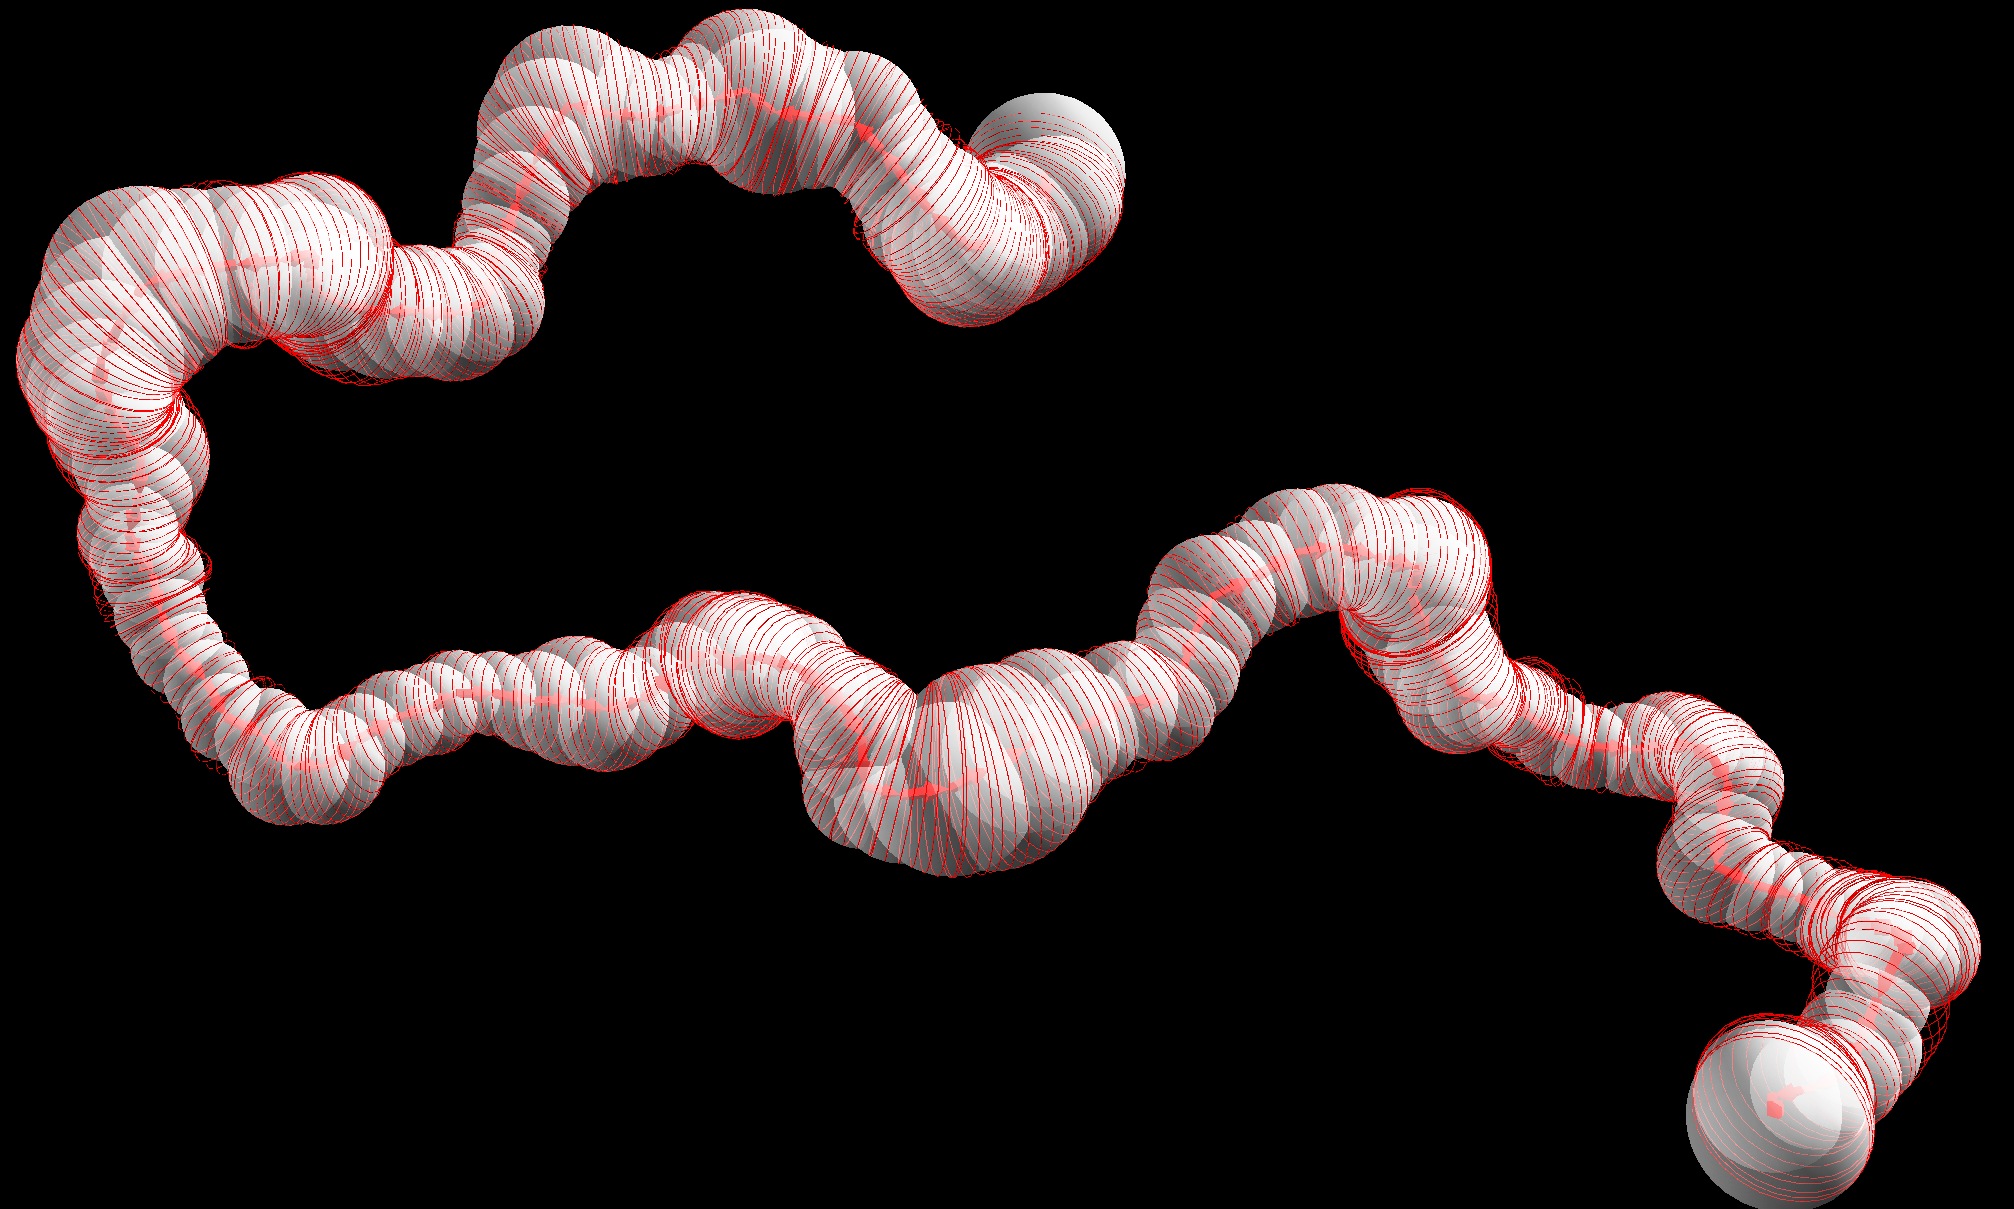
\includegraphics[width=.75\textwidth]{img/1YGE.png}
    \caption{Diskretizace tunelu v enzymu Lipooxygenase (1YGE).}
  \centering
  \label{fig:1YGE}
\end{figure}

\begin{figure}[ht]
    \centering
    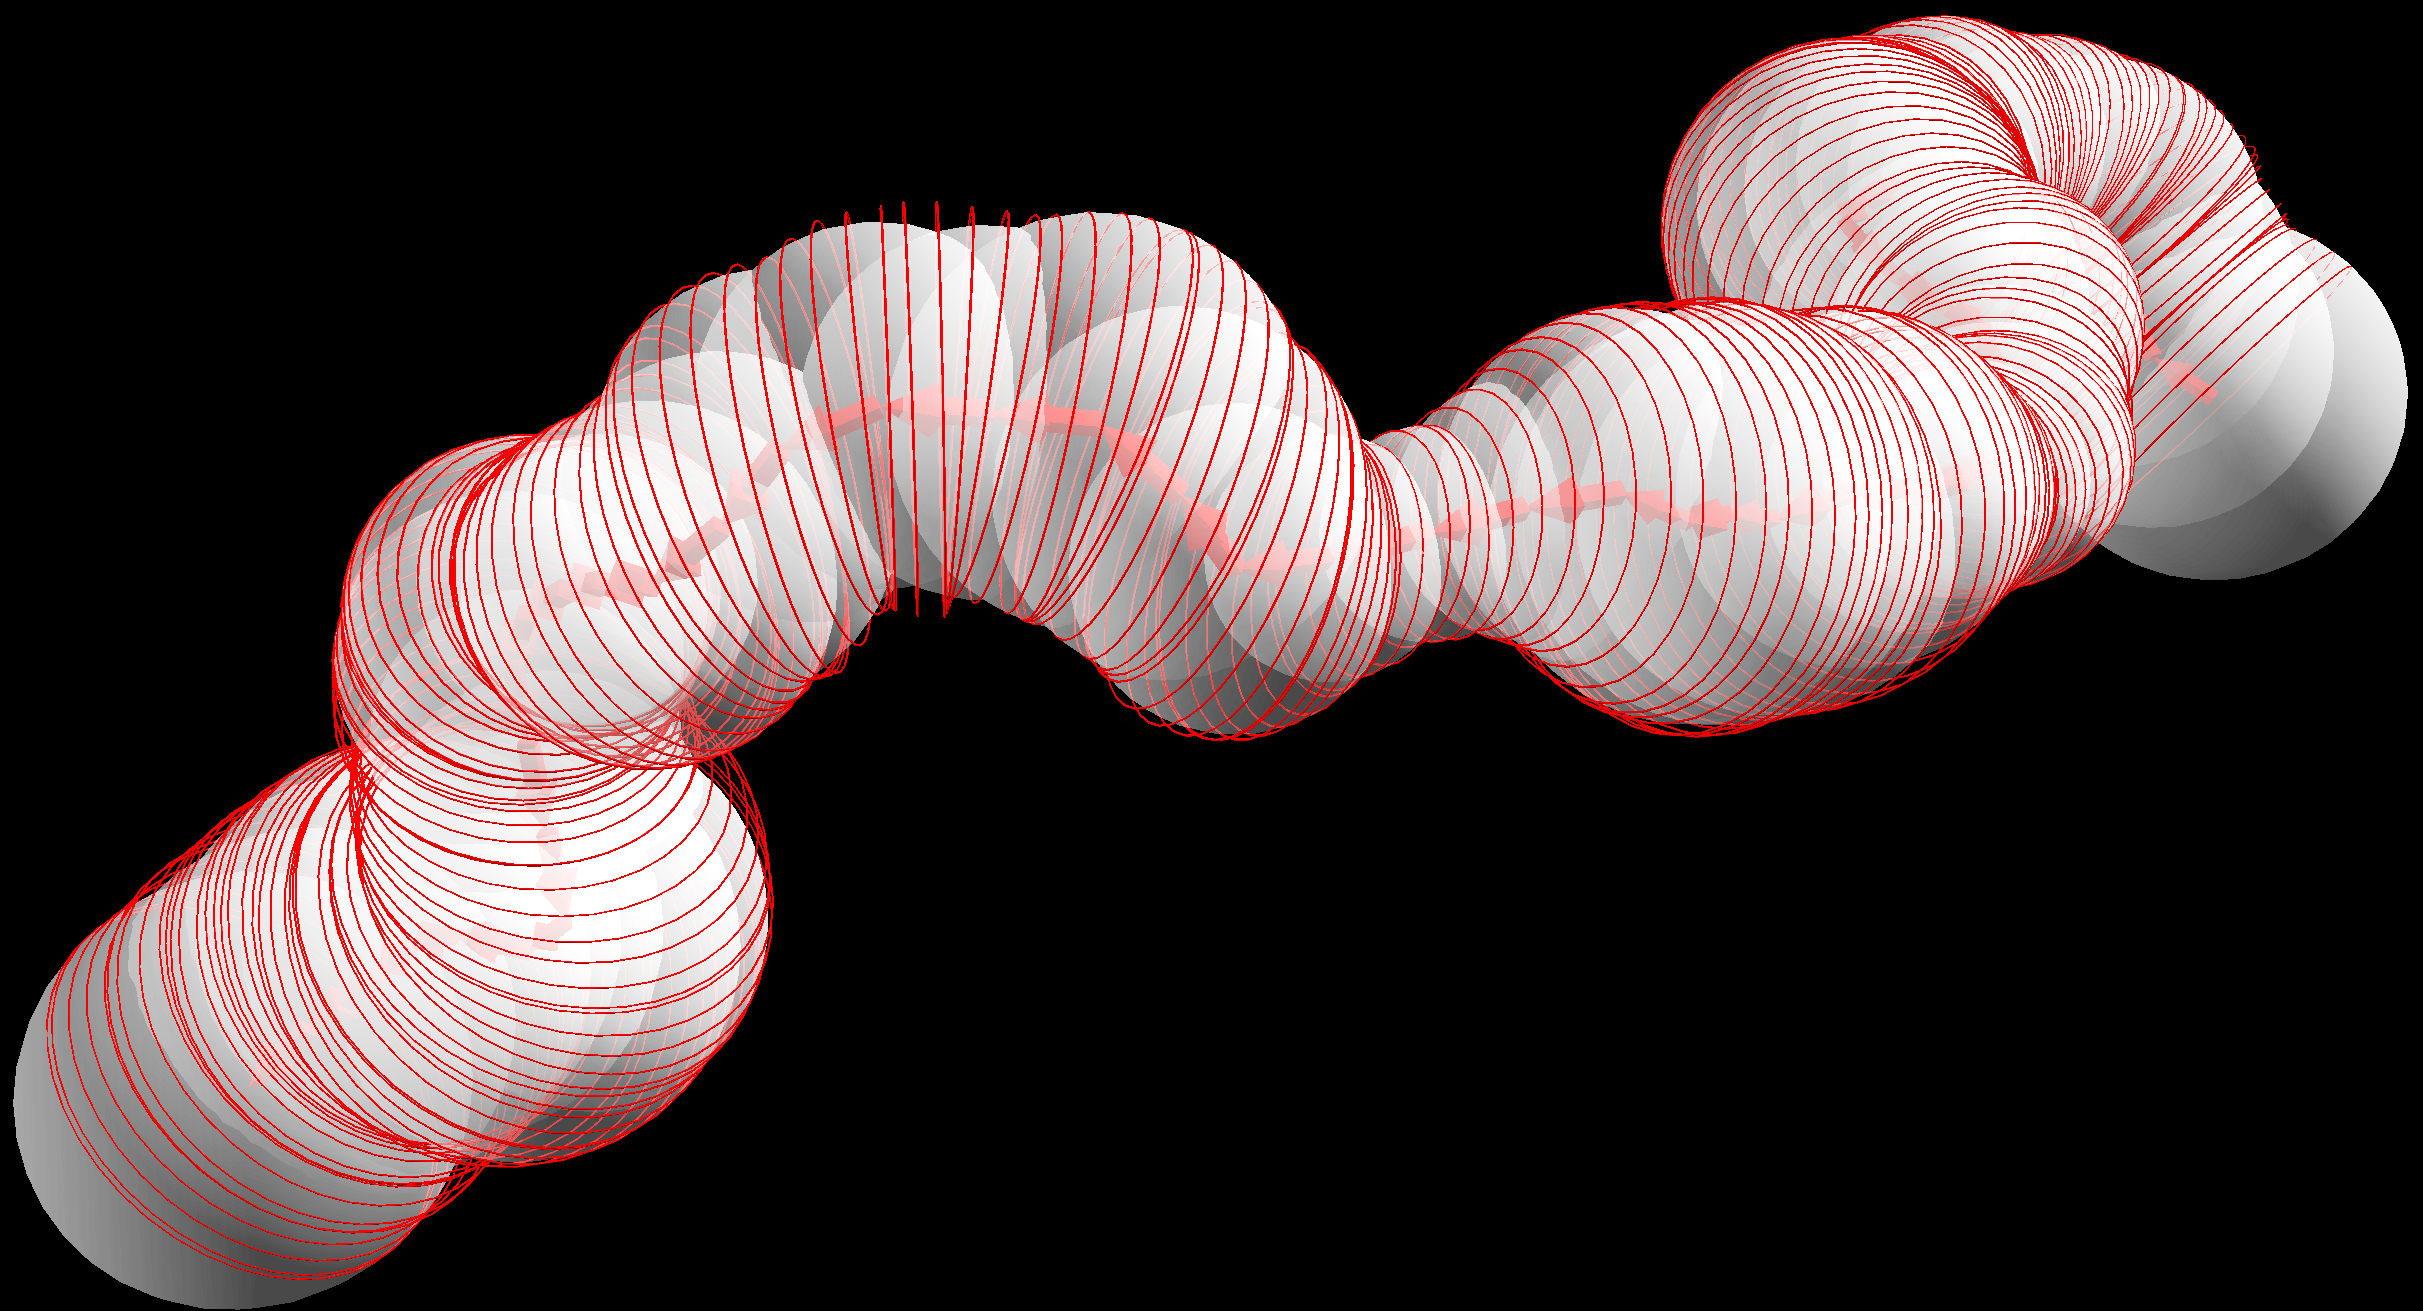
\includegraphics[width=.75\textwidth]{img/2INC.png}
    \caption{Diskretizace tunelu v enzymu  Toluene/o-xylene monooxygenase (2INC).}
  \centering
  \label{fig:2INC}
\end{figure}

\begin{figure}[ht]
\centering
\begin{minipage}{.5\textwidth}
  \centering
    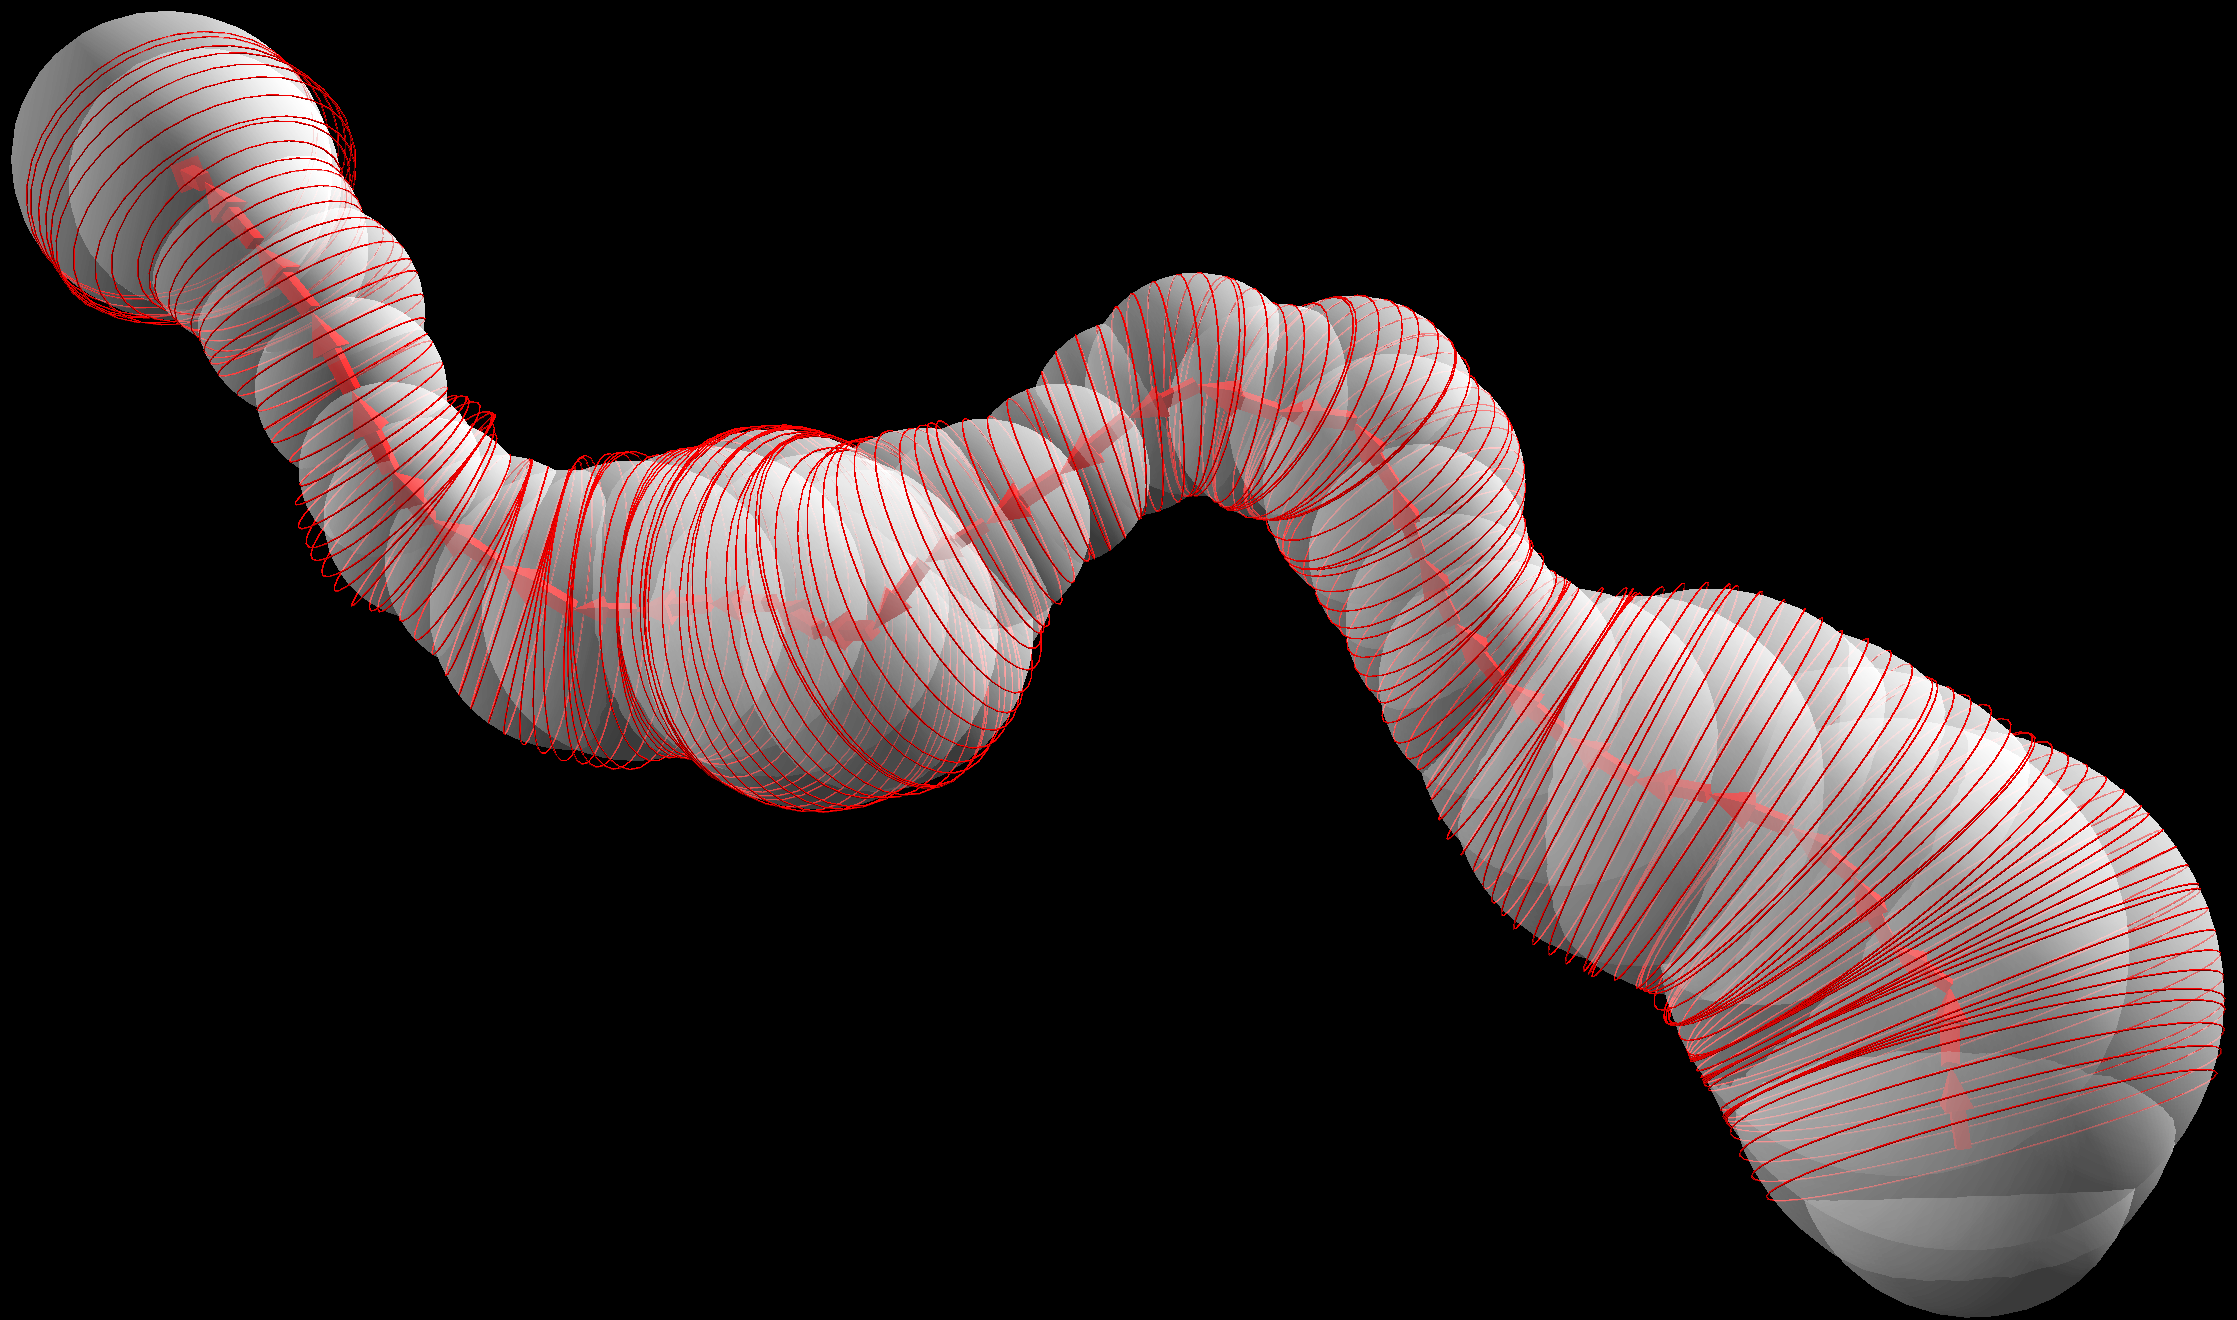
\includegraphics[width=70mm]{img/1EA5.png}
    \caption{Acetylcholinesterase (1EA5).}
  \centering
  \label{fig:1EA5}
\end{minipage}%
\begin{minipage}{.5\textwidth}
     \centering
    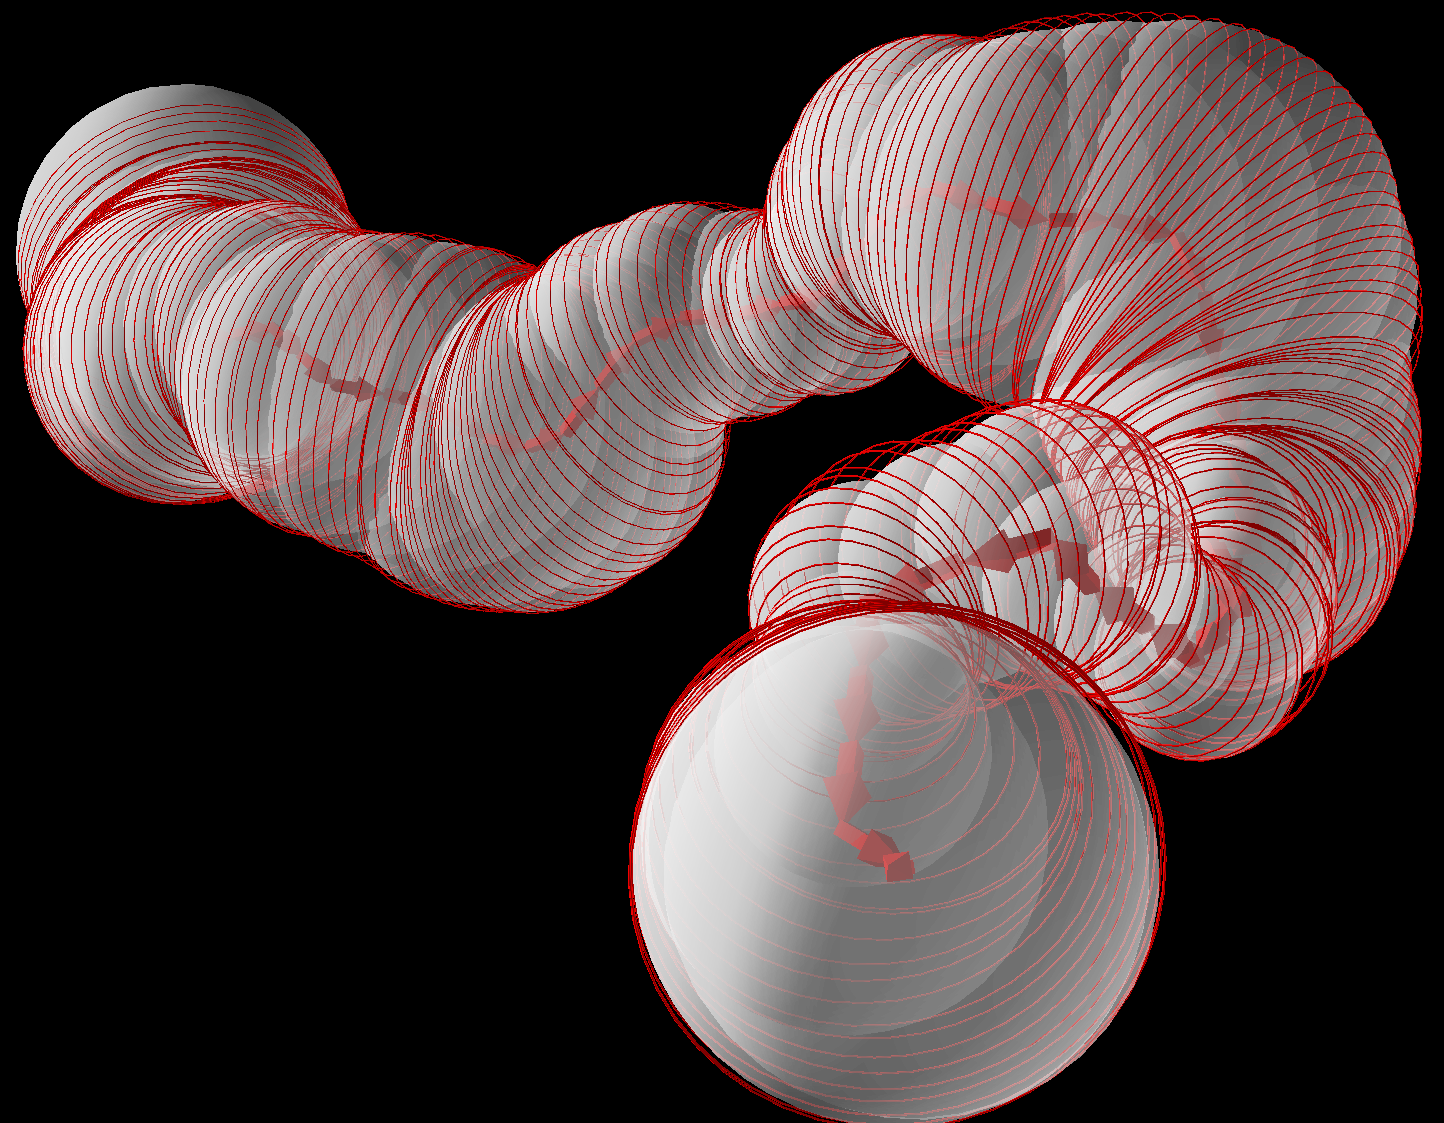
\includegraphics[width=70mm]{img/2SQC.png}
    \caption{Squalene-hopene cyclase (2SQC).}
  \centering
  \label{fig:2SQC}
\end{minipage}
\end{figure}
